% lecture5.tex -- GENERATED by build_L5.py from L5_numbers.json; do not edit by hand.
\documentclass[10pt,aspectratio=169,t]{beamer}
% =============================================================================
% nn_preamble.tex -- shared Beamer preamble of Neural Networks and Deep Learning (NN)
% Used by every lecture: lectures/Lk/lecturek.tex does
%   \documentclass[10pt,aspectratio=169,t]{beamer}
%   % =============================================================================
% nn_preamble.tex -- shared Beamer preamble of Neural Networks and Deep Learning (NN)
% Used by every lecture: lectures/Lk/lecturek.tex does
%   \documentclass[10pt,aspectratio=169,t]{beamer}
%   % =============================================================================
% nn_preamble.tex -- shared Beamer preamble of Neural Networks and Deep Learning (NN)
% Used by every lecture: lectures/Lk/lecturek.tex does
%   \documentclass[10pt,aspectratio=169,t]{beamer}
%   \input{../common/nn_preamble}
%   \nnlecture{k}{Lecture title}
% Logos live in lectures/common/logos/, charts in lectures/Lk/charts/.
% Do NOT add \hfuzz / \vfuzz / \hbadness here: overfull boxes must be fixed, not hidden.
% =============================================================================

\usetheme{default}
\setbeamersize{text margin left=7mm, text margin right=7mm}

% ---------------------------------------------------------------- packages
\usepackage[utf8]{inputenc}
\usepackage[T1]{fontenc}
\usepackage{lmodern}
\usepackage{amsmath, amssymb}
\usepackage{mathtools}
\usepackage{bm}
\usepackage{tikz}
\usetikzlibrary{arrows.meta, positioning, calc, shapes.misc}
\usepackage{booktabs}
\usepackage{array}
\usepackage{graphicx}
\usepackage{colortbl}
\usepackage{xcolor}
\usepackage{multicol}
\hypersetup{colorlinks=true, linkcolor=MainBlue, urlcolor=MainBlue, citecolor=MainBlue}
\graphicspath{{../common/logos/}}   % charts are included with their language folder: charts/en/, charts/ro/

% ---------------------------------------------------------------- colours
\definecolor{MainBlue}{RGB}{26, 58, 110}
\definecolor{IDAred}{RGB}{205, 0, 0}
\definecolor{DarkGray}{RGB}{51, 51, 51}
\definecolor{FooterGray}{RGB}{100, 100, 100}
\definecolor{BlockGray}{RGB}{236, 238, 242}
\definecolor{KeynoteGray}{RGB}{218, 218, 218}
\definecolor{Crimson}{RGB}{190, 40, 50}
\definecolor{Forest}{RGB}{30, 110, 50}
\definecolor{Bitter}{RGB}{214, 150, 20}
% chart palette (same hex values and order as lectures/common/nn_plot.py SERIES)
\definecolor{Ser1}{HTML}{2A78D6}
\definecolor{Ser2}{HTML}{EB6834}
\definecolor{Ser3}{HTML}{1BAF7A}
\definecolor{Ser4}{HTML}{EDA100}
\definecolor{Ser5}{HTML}{E87BA4}
\definecolor{Ser6}{HTML}{008300}
\definecolor{Ser7}{HTML}{6250D6}
\definecolor{Ser8}{HTML}{E34948}

\setbeamertemplate{background}{%
  \begin{tikzpicture}[remember picture, overlay]
    \shade[shading=axis, shading angle=315, top color=white, bottom color=KeynoteGray]
      (current page.south west) rectangle (current page.north east);
  \end{tikzpicture}}
\setbeamercolor{background canvas}{bg=}
\setbeamercolor{structure}{fg=MainBlue}
\setbeamercolor{normal text}{fg=DarkGray}
\setbeamercolor{title}{fg=IDAred}
\setbeamercolor{frametitle}{fg=IDAred, bg=}
\setbeamercolor{block title}{bg=MainBlue, fg=white}
\setbeamercolor{block body}{bg=BlockGray, fg=DarkGray}
\setbeamercolor{block title alerted}{bg=Crimson, fg=white}
\setbeamercolor{block body alerted}{bg=Crimson!7, fg=DarkGray}
\setbeamercolor{block title example}{bg=Forest, fg=white}
\setbeamercolor{block body example}{bg=Forest!7, fg=DarkGray}
\setbeamercolor{item}{fg=MainBlue}
\setbeamerfont{frametitle}{size=\large, series=\bfseries}
\setbeamerfont{block title}{size=\small, series=\bfseries}
\setbeamertemplate{blocks}[rounded][shadow=false]
\setbeamertemplate{itemize item}{\color{MainBlue}$\boxdot$}
\setbeamertemplate{itemize subitem}{\color{MainBlue}\scriptsize$\blacktriangleright$}
% compact two-level lists: level 1 = main point, level 2 = details (no text outside bullets)
\setbeamerfont{itemize/enumerate subbody}{size=\footnotesize}
\setlength{\leftmargini}{1.1em}
\setlength{\leftmarginii}{1.1em}
\setbeamertemplate{itemize/enumerate body begin}{\setlength{\topsep}{0pt}\setlength{\partopsep}{0pt}\setlength{\parskip}{0pt}}
\setbeamertemplate{itemize/enumerate subbody begin}{\setlength{\topsep}{0pt}\setlength{\partopsep}{0pt}\setlength{\itemsep}{0pt}\vspace{-0.4ex}}

\setbeamertemplate{enumerate item}{\color{MainBlue}\insertenumlabel.}
\setlength{\leftmargini}{1.3em}
\setlength{\leftmarginii}{1.2em}
\setbeamertemplate{navigation symbols}{}
\setbeamertemplate{section in toc}{\color{MainBlue}$\blacktriangleright$~\inserttocsection}
\setbeamertemplate{caption}{\raggedright\insertcaption\par}
% frame subtitle = precise citation line under the claim title (Weron style)
\setbeamerfont{framesubtitle}{size=\footnotesize}
\setbeamercolor{framesubtitle}{fg=FooterGray}
% outline that reappears at every section with the current section highlighted
\setbeamertemplate{section in toc shaded}[default][35]
\setbeamertemplate{subsection in toc shaded}[default][35]
\setbeamertemplate{subsection in toc}{\leavevmode\leftskip=2.2em\color{DarkGray}\small\inserttocsubsection\par}
\AtBeginSection[]{{\begin{frame}{\txtoutline}\vspace{2mm}\small
  \tableofcontents[currentsection,hideothersubsections]\end{frame}}}

% ---------------------------------------------------------------- head and foot
\setbeamertemplate{headline}{%
  \vskip10pt%
  \hbox to \paperwidth{\hskip0.5cm%
    {\small\color{FooterGray}\renewcommand{\hyperlink}[2]{##2}\insertsectionhead}%
    \hfill\textcolor{FooterGray}{\small\insertframenumber}\hskip0.5cm}%
  \vskip4pt{\color{FooterGray}\hrule height 0.4pt}}
% footer as in the other courses (MFM, SFM): course name on the left, small sparkline on the right
\setbeamertemplate{footline}{%
  {\color{FooterGray}\hrule height 0.4pt}\vskip4pt%
  \hbox to \paperwidth{\hskip0.5cm%
    \textcolor{FooterGray}{\small\txtcourse}%
    \hfill\raisebox{-0.1em}{\begin{tikzpicture}[x=0.08em, y=0.08em, line width=0.4pt]
      \draw[FooterGray] (0,3) -- (1,4) -- (2,3.5) -- (3,5) -- (4,4) -- (5,6) -- (6,5.5) -- (7,4) -- (8,5) -- (9,7) -- (10,6) -- (11,5) -- (12,6.5) -- (13,8) -- (14,7) -- (15,6) -- (16,7.5) -- (17,9) -- (18,8) -- (19,7) -- (20,8.5) -- (21,10) -- (22,9) -- (23,8) -- (24,9.5);
    \end{tikzpicture}}\hskip0.5cm}%
  \vskip6pt}

% ---------------------------------------------------------------- title page
\defbeamertemplate*{title page}{nn}[1][]{%
  \vspace{0.15cm}
  \begin{center}
    \href{https://www.ase.ro}{
\includegraphics[height=0.9cm]{ase_logo.png}}\hspace{0.3cm}%
    \href{https://ipe.ro/new}{
\includegraphics[height=0.9cm]{acad_logo.png}}\hspace{0.3cm}%
    \href{https://theida.net}{
\includegraphics[height=0.9cm]{ida_logo.png}}\hspace{0.3cm}%
    \href{https://blockchain-research-center.com}{
\includegraphics[height=0.9cm]{brc_logo.png}}\hspace{0.3cm}%
    \href{https://www.ai4efin.ase.ro}{
\includegraphics[height=0.9cm]{ai4efin_logo.png}}\hspace{0.3cm}%
    \href{https://www.digital-finance-msca.com}{
\includegraphics[height=0.9cm]{msca_logo.png}}%
  \end{center}
  \vspace{0.45cm}
  \begin{center}
    \begin{minipage}{0.1\textwidth}\centering
      \href{https://quantlet.com}{
\includegraphics[height=0.9cm]{ql_logo.png}}\end{minipage}%
    \begin{minipage}{0.78\textwidth}\centering
      {\Large\bfseries\usebeamercolor[fg]{title}\inserttitle}\par\vspace{0.25cm}
      {\large\usebeamercolor[fg]{title}\insertsubtitle}\end{minipage}%
    \begin{minipage}{0.1\textwidth}\centering
      \href{https://quantinar.com}{
\includegraphics[height=0.9cm]{qr_logo.png}}\end{minipage}
  \end{center}
  \vfill
  \hspace{0.4cm}{\bfseries\insertauthor}\par\vspace{0.12cm}
  \hspace{0.4cm}\begin{minipage}[t]{0.92\textwidth}\raggedright\footnotesize\insertinstitute\end{minipage}
  \par\vspace{0.4cm}}

% ---------------------------------------------------------------- lecture metadata
\newcommand{\nnshort}{}
\newcommand{\nnnb}{notebooks}
\newcommand{\nnrepo}{https://github.com/danpele/NEURAL_BIZ/tree/main}
% language-dependent labels (English default; \nnromanian switches to Romanian, call it before \nnlecture)
\newcommand{\txtcourse}{Neural Networks and Deep Learning}
\newcommand{\txtlecture}{Lecture}
\newcommand{\txtoutline}{Outline}
\newcommand{\txtintuition}{In one sentence:}
\newcommand{\txtjob}{In practice:}
\newcommand{\txttry}{Experiment yourself:}
\newcommand{\txtwhere}{where}
\newcommand{\txtsim}{SIMULATED DATA (teaching illustration)}
\newcommand{\txtnbsuffix}{}
\newcommand{\txtinstitute}{Bucharest University of Economic Studies (ASE), Department of Statistics and Econometrics\\
    Romanian Academy, Institute for Economic Forecasting (IPE)\\
    IDA Institute Digital Assets \textbullet\ AI4EFin \textbullet\ MSCA Digital Finance}
\newcommand{\nnromanian}{%
  \renewcommand{\txtcourse}{Rețele neuronale și deep learning}%
  \renewcommand{\txtlecture}{Cursul}%
  \renewcommand{\txtoutline}{Cuprins}%
  \renewcommand{\txtintuition}{Pe scurt:}%
  \renewcommand{\txtjob}{În practică:}%
  \renewcommand{\txttry}{Exercițiu practic:}%
  \renewcommand{\txtwhere}{unde}%
  \renewcommand{\txtsim}{DATE SIMULATE (doar pentru ilustrare)}%
  \renewcommand{\txtnbsuffix}{\string_ro}%
  \renewcommand{\txtinstitute}{Academia de Studii Economice din București (ASE), Departamentul de Statistică și Econometrie\\
    Academia Română, Institutul de Prognoză Economică (IPE)\\
    IDA Institute Digital Assets \textbullet\ AI4EFin \textbullet\ MSCA Digital Finance}}
\newcommand{\nnlecture}[2]{%
  \renewcommand{\nnshort}{\txtlecture\ #1}%
  \renewcommand{\nnnb}{notebooks/L#1\string_notebook\txtnbsuffix.ipynb}%
  \title[NN]{\txtcourse}%
  \subtitle{\txtlecture\ #1: #2}%
  \author{Prof.\ dr.\ Daniel Traian PELE}%
  \institute{\txtinstitute}%
  \date{}}

% ---------------------------------------------------------------- teaching blocks (one message per frame)
% \intuition{one plain sentence}  ->  formula with every symbol defined  ->  real-data example  ->  \manager{one line}
\newcommand{\intuition}[1]{\begin{itemize}\item {\color{MainBlue}\textbf{\txtintuition}}~#1\end{itemize}\vspace{0.6mm}}
\newcommand{\manager}[1]{\colorbox{Forest!10}{\parbox{\dimexpr\linewidth-2\fboxsep\relax}{\footnotesize
  \begin{itemize}\setlength{\itemsep}{0pt}\item \textbf{\color{Forest}\txtjob}~#1\end{itemize}}}}
% Experiment yourself: pointer to the matching notebook section
\newcommand{\tryit}[1]{{\scriptsize\href{\nnrepo/\nnnb}{%
  \raisebox{-0.15em}{
\includegraphics[height=0.85em]{ql_logo.png}}\,\textbf{\txttry}~\color{MainBlue}#1}}}
% bottom row: manager line (left) + experiment pointer (right), pinned to the bottom of the frame
\newcommand{\bottomrow}[2]{\par\vfill\noindent\begin{minipage}[b]{0.72\linewidth}#1\end{minipage}\hfill
  \begin{minipage}[b]{0.26\linewidth}\raggedleft #2\end{minipage}\par\vspace{0.5mm}}
\newcommand{\where}[1]{{\footnotesize\textbf{\txtwhere}~#1\par}}

% ---------------------------------------------------------------- helpers
% chart source line under a figure: \chartsource{Source ...; period ...}
\newcommand{\chartsource}[1]{\par\vspace{1pt}{\scriptsize\color{FooterGray}#1\par}}
% link to code: \quantlet{label}{path inside the repo}
\newcommand{\quantlet}[2]{\par\vspace{1pt}\hfill\href{\nnrepo/#2}{%
  \raisebox{-0.15em}{
\includegraphics[height=0.75em]{ql_logo.png}}\textcolor{MainBlue}{\scriptsize\ #1}}}
% inline Quantlet link for the bottom-right corner of a frame: \qlink{label}{path inside the repo}
\newcommand{\qlink}[2]{{\scriptsize\href{\nnrepo/#2}{\raisebox{-0.15em}{
\includegraphics[height=0.85em]{ql_logo.png}}\,\textcolor{MainBlue}{#1}}}}
\newcommand{\simlabel}{\colorbox{Crimson!12}{\scriptsize\bfseries\color{Crimson}\txtsim}}
\newcommand{\E}{\mathbb{E}}
\newcommand{\Var}{\operatorname{Var}}
\newcommand{\Cov}{\operatorname{Cov}}
\newcommand{\Corr}{\operatorname{Corr}}
\newcommand{\asinh}{\operatorname{asinh}}
\newcommand{\iid}{\overset{\text{i.i.d.}}{\sim}}
\newcommand{\EUR}{EUR}
% deep-learning notation (Bishop & Bishop, 2024): vectors bold lower case, matrices bold upper case
\newcommand{\R}{\mathbb{R}}
\newcommand{\vx}{\mathbf{x}}
\newcommand{\vy}{\mathbf{y}}
\newcommand{\vz}{\mathbf{z}}
\newcommand{\vh}{\mathbf{h}}
\newcommand{\vw}{\mathbf{w}}
\newcommand{\vb}{\mathbf{b}}
\newcommand{\mW}{\mathbf{W}}
\newcommand{\mX}{\mathbf{X}}
\newcommand{\btheta}{\boldsymbol{\theta}}
\newcommand{\loss}{\mathcal{L}}
\newcommand{\dataset}{\mathcal{D}}
\DeclareMathOperator*{\argmin}{arg\,min}
\DeclareMathOperator*{\argmax}{arg\,max}
\DeclareMathOperator{\softmax}{softmax}
\DeclareMathOperator{\ReLU}{ReLU}
\DeclareMathOperator{\sigm}{\sigma}

%   \nnlecture{k}{Lecture title}
% Logos live in lectures/common/logos/, charts in lectures/Lk/charts/.
% Do NOT add \hfuzz / \vfuzz / \hbadness here: overfull boxes must be fixed, not hidden.
% =============================================================================

\usetheme{default}
\setbeamersize{text margin left=7mm, text margin right=7mm}

% ---------------------------------------------------------------- packages
\usepackage[utf8]{inputenc}
\usepackage[T1]{fontenc}
\usepackage{lmodern}
\usepackage{amsmath, amssymb}
\usepackage{mathtools}
\usepackage{bm}
\usepackage{tikz}
\usetikzlibrary{arrows.meta, positioning, calc, shapes.misc}
\usepackage{booktabs}
\usepackage{array}
\usepackage{graphicx}
\usepackage{colortbl}
\usepackage{xcolor}
\usepackage{multicol}
\hypersetup{colorlinks=true, linkcolor=MainBlue, urlcolor=MainBlue, citecolor=MainBlue}
\graphicspath{{../common/logos/}}   % charts are included with their language folder: charts/en/, charts/ro/

% ---------------------------------------------------------------- colours
\definecolor{MainBlue}{RGB}{26, 58, 110}
\definecolor{IDAred}{RGB}{205, 0, 0}
\definecolor{DarkGray}{RGB}{51, 51, 51}
\definecolor{FooterGray}{RGB}{100, 100, 100}
\definecolor{BlockGray}{RGB}{236, 238, 242}
\definecolor{KeynoteGray}{RGB}{218, 218, 218}
\definecolor{Crimson}{RGB}{190, 40, 50}
\definecolor{Forest}{RGB}{30, 110, 50}
\definecolor{Bitter}{RGB}{214, 150, 20}
% chart palette (same hex values and order as lectures/common/nn_plot.py SERIES)
\definecolor{Ser1}{HTML}{2A78D6}
\definecolor{Ser2}{HTML}{EB6834}
\definecolor{Ser3}{HTML}{1BAF7A}
\definecolor{Ser4}{HTML}{EDA100}
\definecolor{Ser5}{HTML}{E87BA4}
\definecolor{Ser6}{HTML}{008300}
\definecolor{Ser7}{HTML}{6250D6}
\definecolor{Ser8}{HTML}{E34948}

\setbeamertemplate{background}{%
  \begin{tikzpicture}[remember picture, overlay]
    \shade[shading=axis, shading angle=315, top color=white, bottom color=KeynoteGray]
      (current page.south west) rectangle (current page.north east);
  \end{tikzpicture}}
\setbeamercolor{background canvas}{bg=}
\setbeamercolor{structure}{fg=MainBlue}
\setbeamercolor{normal text}{fg=DarkGray}
\setbeamercolor{title}{fg=IDAred}
\setbeamercolor{frametitle}{fg=IDAred, bg=}
\setbeamercolor{block title}{bg=MainBlue, fg=white}
\setbeamercolor{block body}{bg=BlockGray, fg=DarkGray}
\setbeamercolor{block title alerted}{bg=Crimson, fg=white}
\setbeamercolor{block body alerted}{bg=Crimson!7, fg=DarkGray}
\setbeamercolor{block title example}{bg=Forest, fg=white}
\setbeamercolor{block body example}{bg=Forest!7, fg=DarkGray}
\setbeamercolor{item}{fg=MainBlue}
\setbeamerfont{frametitle}{size=\large, series=\bfseries}
\setbeamerfont{block title}{size=\small, series=\bfseries}
\setbeamertemplate{blocks}[rounded][shadow=false]
\setbeamertemplate{itemize item}{\color{MainBlue}$\boxdot$}
\setbeamertemplate{itemize subitem}{\color{MainBlue}\scriptsize$\blacktriangleright$}
% compact two-level lists: level 1 = main point, level 2 = details (no text outside bullets)
\setbeamerfont{itemize/enumerate subbody}{size=\footnotesize}
\setlength{\leftmargini}{1.1em}
\setlength{\leftmarginii}{1.1em}
\setbeamertemplate{itemize/enumerate body begin}{\setlength{\topsep}{0pt}\setlength{\partopsep}{0pt}\setlength{\parskip}{0pt}}
\setbeamertemplate{itemize/enumerate subbody begin}{\setlength{\topsep}{0pt}\setlength{\partopsep}{0pt}\setlength{\itemsep}{0pt}\vspace{-0.4ex}}

\setbeamertemplate{enumerate item}{\color{MainBlue}\insertenumlabel.}
\setlength{\leftmargini}{1.3em}
\setlength{\leftmarginii}{1.2em}
\setbeamertemplate{navigation symbols}{}
\setbeamertemplate{section in toc}{\color{MainBlue}$\blacktriangleright$~\inserttocsection}
\setbeamertemplate{caption}{\raggedright\insertcaption\par}
% frame subtitle = precise citation line under the claim title (Weron style)
\setbeamerfont{framesubtitle}{size=\footnotesize}
\setbeamercolor{framesubtitle}{fg=FooterGray}
% outline that reappears at every section with the current section highlighted
\setbeamertemplate{section in toc shaded}[default][35]
\setbeamertemplate{subsection in toc shaded}[default][35]
\setbeamertemplate{subsection in toc}{\leavevmode\leftskip=2.2em\color{DarkGray}\small\inserttocsubsection\par}
\AtBeginSection[]{{\begin{frame}{\txtoutline}\vspace{2mm}\small
  \tableofcontents[currentsection,hideothersubsections]\end{frame}}}

% ---------------------------------------------------------------- head and foot
\setbeamertemplate{headline}{%
  \vskip10pt%
  \hbox to \paperwidth{\hskip0.5cm%
    {\small\color{FooterGray}\renewcommand{\hyperlink}[2]{##2}\insertsectionhead}%
    \hfill\textcolor{FooterGray}{\small\insertframenumber}\hskip0.5cm}%
  \vskip4pt{\color{FooterGray}\hrule height 0.4pt}}
% footer as in the other courses (MFM, SFM): course name on the left, small sparkline on the right
\setbeamertemplate{footline}{%
  {\color{FooterGray}\hrule height 0.4pt}\vskip4pt%
  \hbox to \paperwidth{\hskip0.5cm%
    \textcolor{FooterGray}{\small\txtcourse}%
    \hfill\raisebox{-0.1em}{\begin{tikzpicture}[x=0.08em, y=0.08em, line width=0.4pt]
      \draw[FooterGray] (0,3) -- (1,4) -- (2,3.5) -- (3,5) -- (4,4) -- (5,6) -- (6,5.5) -- (7,4) -- (8,5) -- (9,7) -- (10,6) -- (11,5) -- (12,6.5) -- (13,8) -- (14,7) -- (15,6) -- (16,7.5) -- (17,9) -- (18,8) -- (19,7) -- (20,8.5) -- (21,10) -- (22,9) -- (23,8) -- (24,9.5);
    \end{tikzpicture}}\hskip0.5cm}%
  \vskip6pt}

% ---------------------------------------------------------------- title page
\defbeamertemplate*{title page}{nn}[1][]{%
  \vspace{0.15cm}
  \begin{center}
    \href{https://www.ase.ro}{
\includegraphics[height=0.9cm]{ase_logo.png}}\hspace{0.3cm}%
    \href{https://ipe.ro/new}{
\includegraphics[height=0.9cm]{acad_logo.png}}\hspace{0.3cm}%
    \href{https://theida.net}{
\includegraphics[height=0.9cm]{ida_logo.png}}\hspace{0.3cm}%
    \href{https://blockchain-research-center.com}{
\includegraphics[height=0.9cm]{brc_logo.png}}\hspace{0.3cm}%
    \href{https://www.ai4efin.ase.ro}{
\includegraphics[height=0.9cm]{ai4efin_logo.png}}\hspace{0.3cm}%
    \href{https://www.digital-finance-msca.com}{
\includegraphics[height=0.9cm]{msca_logo.png}}%
  \end{center}
  \vspace{0.45cm}
  \begin{center}
    \begin{minipage}{0.1\textwidth}\centering
      \href{https://quantlet.com}{
\includegraphics[height=0.9cm]{ql_logo.png}}\end{minipage}%
    \begin{minipage}{0.78\textwidth}\centering
      {\Large\bfseries\usebeamercolor[fg]{title}\inserttitle}\par\vspace{0.25cm}
      {\large\usebeamercolor[fg]{title}\insertsubtitle}\end{minipage}%
    \begin{minipage}{0.1\textwidth}\centering
      \href{https://quantinar.com}{
\includegraphics[height=0.9cm]{qr_logo.png}}\end{minipage}
  \end{center}
  \vfill
  \hspace{0.4cm}{\bfseries\insertauthor}\par\vspace{0.12cm}
  \hspace{0.4cm}\begin{minipage}[t]{0.92\textwidth}\raggedright\footnotesize\insertinstitute\end{minipage}
  \par\vspace{0.4cm}}

% ---------------------------------------------------------------- lecture metadata
\newcommand{\nnshort}{}
\newcommand{\nnnb}{notebooks}
\newcommand{\nnrepo}{https://github.com/danpele/NEURAL_BIZ/tree/main}
% language-dependent labels (English default; \nnromanian switches to Romanian, call it before \nnlecture)
\newcommand{\txtcourse}{Neural Networks and Deep Learning}
\newcommand{\txtlecture}{Lecture}
\newcommand{\txtoutline}{Outline}
\newcommand{\txtintuition}{In one sentence:}
\newcommand{\txtjob}{In practice:}
\newcommand{\txttry}{Experiment yourself:}
\newcommand{\txtwhere}{where}
\newcommand{\txtsim}{SIMULATED DATA (teaching illustration)}
\newcommand{\txtnbsuffix}{}
\newcommand{\txtinstitute}{Bucharest University of Economic Studies (ASE), Department of Statistics and Econometrics\\
    Romanian Academy, Institute for Economic Forecasting (IPE)\\
    IDA Institute Digital Assets \textbullet\ AI4EFin \textbullet\ MSCA Digital Finance}
\newcommand{\nnromanian}{%
  \renewcommand{\txtcourse}{Rețele neuronale și deep learning}%
  \renewcommand{\txtlecture}{Cursul}%
  \renewcommand{\txtoutline}{Cuprins}%
  \renewcommand{\txtintuition}{Pe scurt:}%
  \renewcommand{\txtjob}{În practică:}%
  \renewcommand{\txttry}{Exercițiu practic:}%
  \renewcommand{\txtwhere}{unde}%
  \renewcommand{\txtsim}{DATE SIMULATE (doar pentru ilustrare)}%
  \renewcommand{\txtnbsuffix}{\string_ro}%
  \renewcommand{\txtinstitute}{Academia de Studii Economice din București (ASE), Departamentul de Statistică și Econometrie\\
    Academia Română, Institutul de Prognoză Economică (IPE)\\
    IDA Institute Digital Assets \textbullet\ AI4EFin \textbullet\ MSCA Digital Finance}}
\newcommand{\nnlecture}[2]{%
  \renewcommand{\nnshort}{\txtlecture\ #1}%
  \renewcommand{\nnnb}{notebooks/L#1\string_notebook\txtnbsuffix.ipynb}%
  \title[NN]{\txtcourse}%
  \subtitle{\txtlecture\ #1: #2}%
  \author{Prof.\ dr.\ Daniel Traian PELE}%
  \institute{\txtinstitute}%
  \date{}}

% ---------------------------------------------------------------- teaching blocks (one message per frame)
% \intuition{one plain sentence}  ->  formula with every symbol defined  ->  real-data example  ->  \manager{one line}
\newcommand{\intuition}[1]{\begin{itemize}\item {\color{MainBlue}\textbf{\txtintuition}}~#1\end{itemize}\vspace{0.6mm}}
\newcommand{\manager}[1]{\colorbox{Forest!10}{\parbox{\dimexpr\linewidth-2\fboxsep\relax}{\footnotesize
  \begin{itemize}\setlength{\itemsep}{0pt}\item \textbf{\color{Forest}\txtjob}~#1\end{itemize}}}}
% Experiment yourself: pointer to the matching notebook section
\newcommand{\tryit}[1]{{\scriptsize\href{\nnrepo/\nnnb}{%
  \raisebox{-0.15em}{
\includegraphics[height=0.85em]{ql_logo.png}}\,\textbf{\txttry}~\color{MainBlue}#1}}}
% bottom row: manager line (left) + experiment pointer (right), pinned to the bottom of the frame
\newcommand{\bottomrow}[2]{\par\vfill\noindent\begin{minipage}[b]{0.72\linewidth}#1\end{minipage}\hfill
  \begin{minipage}[b]{0.26\linewidth}\raggedleft #2\end{minipage}\par\vspace{0.5mm}}
\newcommand{\where}[1]{{\footnotesize\textbf{\txtwhere}~#1\par}}

% ---------------------------------------------------------------- helpers
% chart source line under a figure: \chartsource{Source ...; period ...}
\newcommand{\chartsource}[1]{\par\vspace{1pt}{\scriptsize\color{FooterGray}#1\par}}
% link to code: \quantlet{label}{path inside the repo}
\newcommand{\quantlet}[2]{\par\vspace{1pt}\hfill\href{\nnrepo/#2}{%
  \raisebox{-0.15em}{
\includegraphics[height=0.75em]{ql_logo.png}}\textcolor{MainBlue}{\scriptsize\ #1}}}
% inline Quantlet link for the bottom-right corner of a frame: \qlink{label}{path inside the repo}
\newcommand{\qlink}[2]{{\scriptsize\href{\nnrepo/#2}{\raisebox{-0.15em}{
\includegraphics[height=0.85em]{ql_logo.png}}\,\textcolor{MainBlue}{#1}}}}
\newcommand{\simlabel}{\colorbox{Crimson!12}{\scriptsize\bfseries\color{Crimson}\txtsim}}
\newcommand{\E}{\mathbb{E}}
\newcommand{\Var}{\operatorname{Var}}
\newcommand{\Cov}{\operatorname{Cov}}
\newcommand{\Corr}{\operatorname{Corr}}
\newcommand{\asinh}{\operatorname{asinh}}
\newcommand{\iid}{\overset{\text{i.i.d.}}{\sim}}
\newcommand{\EUR}{EUR}
% deep-learning notation (Bishop & Bishop, 2024): vectors bold lower case, matrices bold upper case
\newcommand{\R}{\mathbb{R}}
\newcommand{\vx}{\mathbf{x}}
\newcommand{\vy}{\mathbf{y}}
\newcommand{\vz}{\mathbf{z}}
\newcommand{\vh}{\mathbf{h}}
\newcommand{\vw}{\mathbf{w}}
\newcommand{\vb}{\mathbf{b}}
\newcommand{\mW}{\mathbf{W}}
\newcommand{\mX}{\mathbf{X}}
\newcommand{\btheta}{\boldsymbol{\theta}}
\newcommand{\loss}{\mathcal{L}}
\newcommand{\dataset}{\mathcal{D}}
\DeclareMathOperator*{\argmin}{arg\,min}
\DeclareMathOperator*{\argmax}{arg\,max}
\DeclareMathOperator{\softmax}{softmax}
\DeclareMathOperator{\ReLU}{ReLU}
\DeclareMathOperator{\sigm}{\sigma}

%   \nnlecture{k}{Lecture title}
% Logos live in lectures/common/logos/, charts in lectures/Lk/charts/.
% Do NOT add \hfuzz / \vfuzz / \hbadness here: overfull boxes must be fixed, not hidden.
% =============================================================================

\usetheme{default}
\setbeamersize{text margin left=7mm, text margin right=7mm}

% ---------------------------------------------------------------- packages
\usepackage[utf8]{inputenc}
\usepackage[T1]{fontenc}
\usepackage{lmodern}
\usepackage{amsmath, amssymb}
\usepackage{mathtools}
\usepackage{bm}
\usepackage{tikz}
\usetikzlibrary{arrows.meta, positioning, calc, shapes.misc}
\usepackage{booktabs}
\usepackage{array}
\usepackage{graphicx}
\usepackage{colortbl}
\usepackage{xcolor}
\usepackage{multicol}
\hypersetup{colorlinks=true, linkcolor=MainBlue, urlcolor=MainBlue, citecolor=MainBlue}
\graphicspath{{../common/logos/}}   % charts are included with their language folder: charts/en/, charts/ro/

% ---------------------------------------------------------------- colours
\definecolor{MainBlue}{RGB}{26, 58, 110}
\definecolor{IDAred}{RGB}{205, 0, 0}
\definecolor{DarkGray}{RGB}{51, 51, 51}
\definecolor{FooterGray}{RGB}{100, 100, 100}
\definecolor{BlockGray}{RGB}{236, 238, 242}
\definecolor{KeynoteGray}{RGB}{218, 218, 218}
\definecolor{Crimson}{RGB}{190, 40, 50}
\definecolor{Forest}{RGB}{30, 110, 50}
\definecolor{Bitter}{RGB}{214, 150, 20}
% chart palette (same hex values and order as lectures/common/nn_plot.py SERIES)
\definecolor{Ser1}{HTML}{2A78D6}
\definecolor{Ser2}{HTML}{EB6834}
\definecolor{Ser3}{HTML}{1BAF7A}
\definecolor{Ser4}{HTML}{EDA100}
\definecolor{Ser5}{HTML}{E87BA4}
\definecolor{Ser6}{HTML}{008300}
\definecolor{Ser7}{HTML}{6250D6}
\definecolor{Ser8}{HTML}{E34948}

\setbeamertemplate{background}{%
  \begin{tikzpicture}[remember picture, overlay]
    \shade[shading=axis, shading angle=315, top color=white, bottom color=KeynoteGray]
      (current page.south west) rectangle (current page.north east);
  \end{tikzpicture}}
\setbeamercolor{background canvas}{bg=}
\setbeamercolor{structure}{fg=MainBlue}
\setbeamercolor{normal text}{fg=DarkGray}
\setbeamercolor{title}{fg=IDAred}
\setbeamercolor{frametitle}{fg=IDAred, bg=}
\setbeamercolor{block title}{bg=MainBlue, fg=white}
\setbeamercolor{block body}{bg=BlockGray, fg=DarkGray}
\setbeamercolor{block title alerted}{bg=Crimson, fg=white}
\setbeamercolor{block body alerted}{bg=Crimson!7, fg=DarkGray}
\setbeamercolor{block title example}{bg=Forest, fg=white}
\setbeamercolor{block body example}{bg=Forest!7, fg=DarkGray}
\setbeamercolor{item}{fg=MainBlue}
\setbeamerfont{frametitle}{size=\large, series=\bfseries}
\setbeamerfont{block title}{size=\small, series=\bfseries}
\setbeamertemplate{blocks}[rounded][shadow=false]
\setbeamertemplate{itemize item}{\color{MainBlue}$\boxdot$}
\setbeamertemplate{itemize subitem}{\color{MainBlue}\scriptsize$\blacktriangleright$}
% compact two-level lists: level 1 = main point, level 2 = details (no text outside bullets)
\setbeamerfont{itemize/enumerate subbody}{size=\footnotesize}
\setlength{\leftmargini}{1.1em}
\setlength{\leftmarginii}{1.1em}
\setbeamertemplate{itemize/enumerate body begin}{\setlength{\topsep}{0pt}\setlength{\partopsep}{0pt}\setlength{\parskip}{0pt}}
\setbeamertemplate{itemize/enumerate subbody begin}{\setlength{\topsep}{0pt}\setlength{\partopsep}{0pt}\setlength{\itemsep}{0pt}\vspace{-0.4ex}}

\setbeamertemplate{enumerate item}{\color{MainBlue}\insertenumlabel.}
\setlength{\leftmargini}{1.3em}
\setlength{\leftmarginii}{1.2em}
\setbeamertemplate{navigation symbols}{}
\setbeamertemplate{section in toc}{\color{MainBlue}$\blacktriangleright$~\inserttocsection}
\setbeamertemplate{caption}{\raggedright\insertcaption\par}
% frame subtitle = precise citation line under the claim title (Weron style)
\setbeamerfont{framesubtitle}{size=\footnotesize}
\setbeamercolor{framesubtitle}{fg=FooterGray}
% outline that reappears at every section with the current section highlighted
\setbeamertemplate{section in toc shaded}[default][35]
\setbeamertemplate{subsection in toc shaded}[default][35]
\setbeamertemplate{subsection in toc}{\leavevmode\leftskip=2.2em\color{DarkGray}\small\inserttocsubsection\par}
\AtBeginSection[]{{\begin{frame}{\txtoutline}\vspace{2mm}\small
  \tableofcontents[currentsection,hideothersubsections]\end{frame}}}

% ---------------------------------------------------------------- head and foot
\setbeamertemplate{headline}{%
  \vskip10pt%
  \hbox to \paperwidth{\hskip0.5cm%
    {\small\color{FooterGray}\renewcommand{\hyperlink}[2]{##2}\insertsectionhead}%
    \hfill\textcolor{FooterGray}{\small\insertframenumber}\hskip0.5cm}%
  \vskip4pt{\color{FooterGray}\hrule height 0.4pt}}
% footer as in the other courses (MFM, SFM): course name on the left, small sparkline on the right
\setbeamertemplate{footline}{%
  {\color{FooterGray}\hrule height 0.4pt}\vskip4pt%
  \hbox to \paperwidth{\hskip0.5cm%
    \textcolor{FooterGray}{\small\txtcourse}%
    \hfill\raisebox{-0.1em}{\begin{tikzpicture}[x=0.08em, y=0.08em, line width=0.4pt]
      \draw[FooterGray] (0,3) -- (1,4) -- (2,3.5) -- (3,5) -- (4,4) -- (5,6) -- (6,5.5) -- (7,4) -- (8,5) -- (9,7) -- (10,6) -- (11,5) -- (12,6.5) -- (13,8) -- (14,7) -- (15,6) -- (16,7.5) -- (17,9) -- (18,8) -- (19,7) -- (20,8.5) -- (21,10) -- (22,9) -- (23,8) -- (24,9.5);
    \end{tikzpicture}}\hskip0.5cm}%
  \vskip6pt}

% ---------------------------------------------------------------- title page
\defbeamertemplate*{title page}{nn}[1][]{%
  \vspace{0.15cm}
  \begin{center}
    \href{https://www.ase.ro}{
\includegraphics[height=0.9cm]{ase_logo.png}}\hspace{0.3cm}%
    \href{https://ipe.ro/new}{
\includegraphics[height=0.9cm]{acad_logo.png}}\hspace{0.3cm}%
    \href{https://theida.net}{
\includegraphics[height=0.9cm]{ida_logo.png}}\hspace{0.3cm}%
    \href{https://blockchain-research-center.com}{
\includegraphics[height=0.9cm]{brc_logo.png}}\hspace{0.3cm}%
    \href{https://www.ai4efin.ase.ro}{
\includegraphics[height=0.9cm]{ai4efin_logo.png}}\hspace{0.3cm}%
    \href{https://www.digital-finance-msca.com}{
\includegraphics[height=0.9cm]{msca_logo.png}}%
  \end{center}
  \vspace{0.45cm}
  \begin{center}
    \begin{minipage}{0.1\textwidth}\centering
      \href{https://quantlet.com}{
\includegraphics[height=0.9cm]{ql_logo.png}}\end{minipage}%
    \begin{minipage}{0.78\textwidth}\centering
      {\Large\bfseries\usebeamercolor[fg]{title}\inserttitle}\par\vspace{0.25cm}
      {\large\usebeamercolor[fg]{title}\insertsubtitle}\end{minipage}%
    \begin{minipage}{0.1\textwidth}\centering
      \href{https://quantinar.com}{
\includegraphics[height=0.9cm]{qr_logo.png}}\end{minipage}
  \end{center}
  \vfill
  \hspace{0.4cm}{\bfseries\insertauthor}\par\vspace{0.12cm}
  \hspace{0.4cm}\begin{minipage}[t]{0.92\textwidth}\raggedright\footnotesize\insertinstitute\end{minipage}
  \par\vspace{0.4cm}}

% ---------------------------------------------------------------- lecture metadata
\newcommand{\nnshort}{}
\newcommand{\nnnb}{notebooks}
\newcommand{\nnrepo}{https://github.com/danpele/NEURAL_BIZ/tree/main}
% language-dependent labels (English default; \nnromanian switches to Romanian, call it before \nnlecture)
\newcommand{\txtcourse}{Neural Networks and Deep Learning}
\newcommand{\txtlecture}{Lecture}
\newcommand{\txtoutline}{Outline}
\newcommand{\txtintuition}{In one sentence:}
\newcommand{\txtjob}{In practice:}
\newcommand{\txttry}{Experiment yourself:}
\newcommand{\txtwhere}{where}
\newcommand{\txtsim}{SIMULATED DATA (teaching illustration)}
\newcommand{\txtnbsuffix}{}
\newcommand{\txtinstitute}{Bucharest University of Economic Studies (ASE), Department of Statistics and Econometrics\\
    Romanian Academy, Institute for Economic Forecasting (IPE)\\
    IDA Institute Digital Assets \textbullet\ AI4EFin \textbullet\ MSCA Digital Finance}
\newcommand{\nnromanian}{%
  \renewcommand{\txtcourse}{Rețele neuronale și deep learning}%
  \renewcommand{\txtlecture}{Cursul}%
  \renewcommand{\txtoutline}{Cuprins}%
  \renewcommand{\txtintuition}{Pe scurt:}%
  \renewcommand{\txtjob}{În practică:}%
  \renewcommand{\txttry}{Exercițiu practic:}%
  \renewcommand{\txtwhere}{unde}%
  \renewcommand{\txtsim}{DATE SIMULATE (doar pentru ilustrare)}%
  \renewcommand{\txtnbsuffix}{\string_ro}%
  \renewcommand{\txtinstitute}{Academia de Studii Economice din București (ASE), Departamentul de Statistică și Econometrie\\
    Academia Română, Institutul de Prognoză Economică (IPE)\\
    IDA Institute Digital Assets \textbullet\ AI4EFin \textbullet\ MSCA Digital Finance}}
\newcommand{\nnlecture}[2]{%
  \renewcommand{\nnshort}{\txtlecture\ #1}%
  \renewcommand{\nnnb}{notebooks/L#1\string_notebook\txtnbsuffix.ipynb}%
  \title[NN]{\txtcourse}%
  \subtitle{\txtlecture\ #1: #2}%
  \author{Prof.\ dr.\ Daniel Traian PELE}%
  \institute{\txtinstitute}%
  \date{}}

% ---------------------------------------------------------------- teaching blocks (one message per frame)
% \intuition{one plain sentence}  ->  formula with every symbol defined  ->  real-data example  ->  \manager{one line}
\newcommand{\intuition}[1]{\begin{itemize}\item {\color{MainBlue}\textbf{\txtintuition}}~#1\end{itemize}\vspace{0.6mm}}
\newcommand{\manager}[1]{\colorbox{Forest!10}{\parbox{\dimexpr\linewidth-2\fboxsep\relax}{\footnotesize
  \begin{itemize}\setlength{\itemsep}{0pt}\item \textbf{\color{Forest}\txtjob}~#1\end{itemize}}}}
% Experiment yourself: pointer to the matching notebook section
\newcommand{\tryit}[1]{{\scriptsize\href{\nnrepo/\nnnb}{%
  \raisebox{-0.15em}{
\includegraphics[height=0.85em]{ql_logo.png}}\,\textbf{\txttry}~\color{MainBlue}#1}}}
% bottom row: manager line (left) + experiment pointer (right), pinned to the bottom of the frame
\newcommand{\bottomrow}[2]{\par\vfill\noindent\begin{minipage}[b]{0.72\linewidth}#1\end{minipage}\hfill
  \begin{minipage}[b]{0.26\linewidth}\raggedleft #2\end{minipage}\par\vspace{0.5mm}}
\newcommand{\where}[1]{{\footnotesize\textbf{\txtwhere}~#1\par}}

% ---------------------------------------------------------------- helpers
% chart source line under a figure: \chartsource{Source ...; period ...}
\newcommand{\chartsource}[1]{\par\vspace{1pt}{\scriptsize\color{FooterGray}#1\par}}
% link to code: \quantlet{label}{path inside the repo}
\newcommand{\quantlet}[2]{\par\vspace{1pt}\hfill\href{\nnrepo/#2}{%
  \raisebox{-0.15em}{
\includegraphics[height=0.75em]{ql_logo.png}}\textcolor{MainBlue}{\scriptsize\ #1}}}
% inline Quantlet link for the bottom-right corner of a frame: \qlink{label}{path inside the repo}
\newcommand{\qlink}[2]{{\scriptsize\href{\nnrepo/#2}{\raisebox{-0.15em}{
\includegraphics[height=0.85em]{ql_logo.png}}\,\textcolor{MainBlue}{#1}}}}
\newcommand{\simlabel}{\colorbox{Crimson!12}{\scriptsize\bfseries\color{Crimson}\txtsim}}
\newcommand{\E}{\mathbb{E}}
\newcommand{\Var}{\operatorname{Var}}
\newcommand{\Cov}{\operatorname{Cov}}
\newcommand{\Corr}{\operatorname{Corr}}
\newcommand{\asinh}{\operatorname{asinh}}
\newcommand{\iid}{\overset{\text{i.i.d.}}{\sim}}
\newcommand{\EUR}{EUR}
% deep-learning notation (Bishop & Bishop, 2024): vectors bold lower case, matrices bold upper case
\newcommand{\R}{\mathbb{R}}
\newcommand{\vx}{\mathbf{x}}
\newcommand{\vy}{\mathbf{y}}
\newcommand{\vz}{\mathbf{z}}
\newcommand{\vh}{\mathbf{h}}
\newcommand{\vw}{\mathbf{w}}
\newcommand{\vb}{\mathbf{b}}
\newcommand{\mW}{\mathbf{W}}
\newcommand{\mX}{\mathbf{X}}
\newcommand{\btheta}{\boldsymbol{\theta}}
\newcommand{\loss}{\mathcal{L}}
\newcommand{\dataset}{\mathcal{D}}
\DeclareMathOperator*{\argmin}{arg\,min}
\DeclareMathOperator*{\argmax}{arg\,max}
\DeclareMathOperator{\softmax}{softmax}
\DeclareMathOperator{\ReLU}{ReLU}
\DeclareMathOperator{\sigm}{\sigma}

\nnlecture{5}{Recurrent networks: RNN, LSTM and GRU for sequences and financial time series}
\begin{document}
{\setbeamertemplate{headline}{}\setbeamertemplate{footline}{}
\begin{frame}\titlepage\end{frame}}
% END-FRONT-MATTER

\begin{frame}{Learning objectives}
\small
\begin{itemize}\setlength{\itemsep}{4pt}
  \item Write a recurrent neural network (RNN) as equations, unroll it in time and count its parameters.
  \item Derive backpropagation through time (BPTT) and explain why gradients vanish or explode.
  \item Read the long short-term memory (LSTM) and gated recurrent unit (GRU) cells gate by gate.
  \item Forecast volatility, returns and electricity load with a leakage-free protocol, after the benchmarks: heterogeneous autoregressive (HAR), generalised autoregressive conditional heteroskedasticity (GARCH), autoregressive (AR) and autoregressive with exogenous inputs (ARX) models.
  \item Explain why a multilayer perceptron (MLP) on a window of past values is not enough.
  \item Decide with a forecast-comparison test when a recurrent network is worth its cost.
\end{itemize}
\end{frame}

% BEGIN-ABBR

\begin{frame}{Abbreviations}
\small
\vspace{-1mm}\begin{columns}[T,onlytextwidth]
\begin{column}{0.49\textwidth}{\scriptsize\renewcommand{\arraystretch}{0.96}\begin{tabular}{@{}>{\bfseries}l@{\ \ }p{0.74\linewidth}@{}}AI & artificial intelligence\\
AR & autoregressive model\\
ARX & autoregressive model with exogenous inputs\\
ASE & Bucharest University of Economic Studies\\
BiLSTM & bidirectional LSTM\\
BPTT & backpropagation through time\\
BVB & Bucharest Stock Exchange\\
CEE & Central and Eastern Europe\\
CNN & convolutional neural network\\
CPU & central processing unit\\
DM & Diebold--Mariano test\\
ENTSO-E & European Network of Transmission System Operators for Electricity\\
EODHD & End of Day Historical Data (data provider)\\
ES & expected shortfall\\
GARCH & generalised autoregressive conditional heteroskedasticity\\\end{tabular}}\end{column}
\begin{column}{0.49\textwidth}{\scriptsize\renewcommand{\arraystretch}{0.96}\begin{tabular}{@{}>{\bfseries}l@{\ \ }p{0.74\linewidth}@{}}GK & Garman--Klass range estimator of variance\\
GRU & gated recurrent unit\\
GW & gigawatt\\
HAR & heterogeneous autoregressive model\\
IPE & Institute for Economic Forecasting, Romanian Academy\\
LSTM & long short-term memory\\
MAE & mean absolute error\\
MAPE & mean absolute percentage error\\
MLP & multilayer perceptron\\
MSE & mean squared error\\
MW & megawatt\\
MWh & megawatt-hour\\
RNN & recurrent neural network\\
TLV & Banca Transilvania (Bucharest Stock Exchange ticker)\\
VaR & value-at-risk\\\end{tabular}}\end{column}
\end{columns}
\end{frame}

% END-ABBR

\begin{frame}{Real data only: three sequences}
\footnotesize
{\footnotesize\renewcommand{\arraystretch}{1.05}\setlength{\tabcolsep}{4pt}
\begin{tabular}{@{}p{0.25\textwidth}p{0.29\textwidth}p{0.22\textwidth}p{0.17\textwidth}@{}}\toprule
Series & Source & Period & Task \\ \midrule
S\&P 500 daily open, high, low, close & Yahoo Finance & 4 Jan 2005 -- 30 Oct 2026 & volatility, returns \\
Banca Transilvania (TLV), adjusted close & End of Day Historical Data (EODHD), Bucharest Stock Exchange (BVB) & 3 Jan 2008 -- 30 Oct 2026 & returns \\
Romanian hourly load & European Network of Transmission System Operators for Electricity (ENTSO-E), via energy-charts.info & 1 Jan 2016 -- 31 Oct 2026 & day-ahead load \\
\bottomrule\end{tabular}}
\par\vspace{0.5mm}{\scriptsize \begin{itemize}\setlength{\itemsep}{0pt}
  \item Time-ordered splits: train to 31 Dec 2016, validation to 31 Dec 2019, test from 1 Jan 2020 (load: train to 31 Dec 2022, validation 31 Dec 2023).
  \item Scalers, early stopping and penalties are fitted on the training or validation years only; the test years are used once.
  \item Networks trained on the central processing unit (CPU), deterministic for a fixed seed (20261108 + seed index).
\end{itemize}}
\par\vfill\noindent{\scriptsize\color{FooterGray}(data/SOURCES.md)}\par\vspace{0.5mm}
\end{frame}


\section{Sequences in finance and energy}

\begin{frame}{Returns look like noise, volatility comes in clusters}
\small
\intuition{the size of the move today says a lot about the size tomorrow; its sign says almost nothing.}
\vspace{-1mm}\[ r_t=100\ln\frac{P_t}{P_{t-1}},\qquad \hat\sigma^2_{\mathrm{GK},t}=\tfrac12\Big(\ln\frac{H_t}{L_t}\Big)^2-(2\ln2-1)\Big(\ln\frac{C_t}{O_t}\Big)^2 \]\vspace{-2mm}
\begin{center}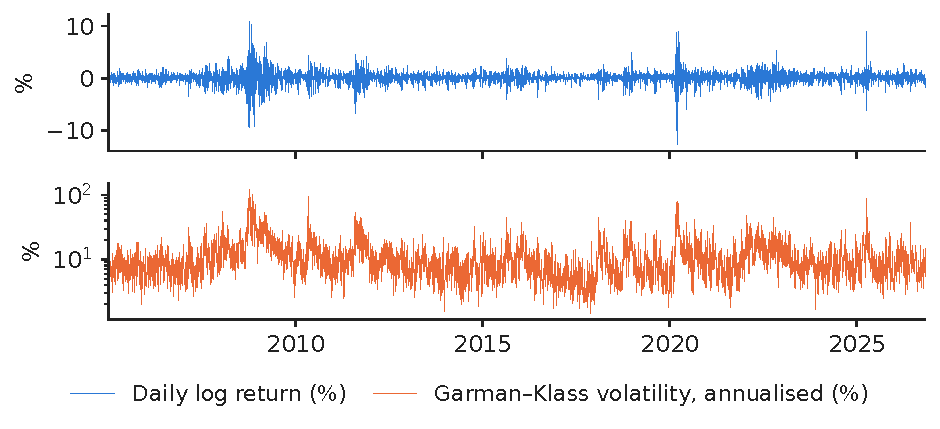
\includegraphics[width=\textwidth,height=0.420\textheight,keepaspectratio]{charts/en/sp500_vol.pdf}\end{center}\vspace{-3mm}
\chartsource{Source: Yahoo Finance, daily quotes. Data: 4 Jan 2005 to 30 Oct 2026, trading days.}
\vspace{0.5mm}
\begin{itemize}\setlength{\itemsep}{0pt}
  \item Garman--Klass (GK) range estimator from open $O_t$, high $H_t$, low $L_t$, close $C_t$
    \begin{itemize}\setlength{\itemsep}{0pt}
      \item Annualised volatility median 8.77\,\%, peak 122\,\% on 10 Oct 2008.
    \end{itemize}
\end{itemize}
\par\vfill\noindent{\scriptsize\color{FooterGray}(Garman \& Klass, 1980; own computation)}\hfill\qlink{NN\_L5\_sp500\_vol}{Quantlets/L5/NN_L5_sp500_vol}\par\vspace{0.5mm}
\end{frame}

\begin{frame}{The memory is in the volatility, not in the returns}
\small
\intuition{autocorrelations of $|r_t|$ stay positive for months; those of $r_t$ are within the noise band.}
\vspace{-1mm}\[ \hat\rho(k)=\frac{\sum_{t=k+1}^{T}(x_t-\bar x)(x_{t-k}-\bar x)}{\sum_{t=1}^{T}(x_t-\bar x)^2} \]\vspace{-2mm}
\begin{center}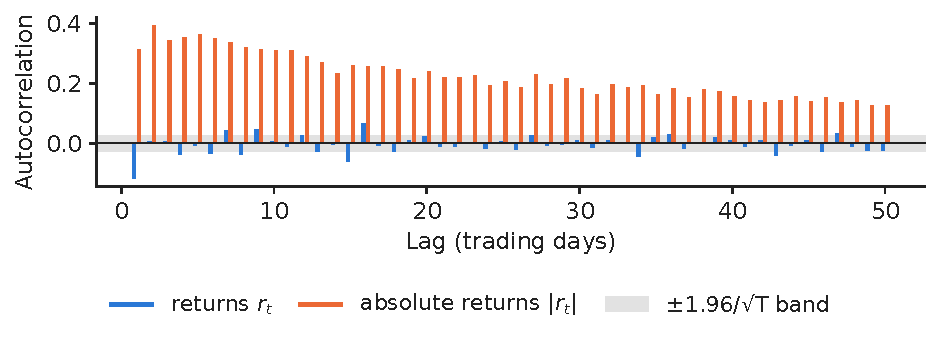
\includegraphics[width=\textwidth,height=0.277\textheight,keepaspectratio]{charts/en/acf_abs.pdf}\end{center}\vspace{-3mm}
\chartsource{Source: Yahoo Finance, daily quotes. Data: 4 Jan 2005 to 30 Oct 2026, trading days.}
\vspace{0.5mm}
\begin{itemize}\setlength{\itemsep}{0pt}
  \item $\hat\rho_r(1)=\ensuremath{-}0.119$ but $\hat\rho_{|r|}(1)=0.315$ and $\hat\rho_{|r|}(50)=0.126$
    \begin{itemize}\setlength{\itemsep}{0pt}
      \item Band $\pm0.026$
      \item Significant lags out of 50: 15 for $r_t$, 50 for $|r_t|$.
    \end{itemize}
\end{itemize}
\par\vfill\manager{a model with memory is worth trying for risk (volatility, value-at-risk (VaR)), much less for the direction of the price.}\par\vspace{0.5mm}
\par\vfill\noindent{\scriptsize\color{FooterGray}(own computation)}\hfill\qlink{NN\_L5\_acf\_abs}{Quantlets/L5/NN_L5_acf_abs}\par\vspace{0.5mm}
\end{frame}

\begin{frame}{A window-MLP forgets everything outside the window}
\footnotesize
\intuition{an MLP on the last $W$ observations has separate weights for every lag and a hard memory limit.}
\begin{columns}[T,onlytextwidth]
\begin{column}{0.53\textwidth}
\[ \hat y_{t+1}=g\big(\mW[\mathbf x_{t-W+1};\dots;\mathbf x_t]+\vb\big),\qquad \mW\in\R^{m\times Wd} \]{\footnotesize\begin{itemize}\setlength{\itemsep}{0pt}
  \item \textbf{\txtwhere}
    \begin{itemize}\setlength{\itemsep}{0pt}
      \item $\mathbf x_t\in\R^d$ the inputs of day $t$
      \item $W$ window length
      \item $m$ hidden units
      \item Parameters grow linearly with $W$
    \end{itemize}
\end{itemize}\par}
\end{column}
\begin{column}{0.44\textwidth}
\begin{itemize}\setlength{\itemsep}{2pt}
  \item \textbf{What we want instead}
    \begin{itemize}\setlength{\itemsep}{0pt}
      \item A state $\vh_t$ that summarises the past
      \item The same update rule at every step (weight sharing in time, like a convolutional neural network (CNN) in space)
      \item Any sequence length
    \end{itemize}
\end{itemize}
\end{column}
\end{columns}
\par\vfill\manager{in production the state is updated with each new observation, without recomputing the whole history.}\par\vspace{0.5mm}
\par\vfill\noindent{\scriptsize\color{FooterGray}(Bishop \& Bishop, 2024, ch.~12)}\par\vspace{0.5mm}
\end{frame}


\section{The recurrent network and backpropagation through time}

\begin{frame}{The vanilla RNN: one state, updated by the same rule}
\footnotesize
\intuition{the new state mixes the old state and the new input through a nonlinearity.}
\begin{columns}[T,onlytextwidth]
\begin{column}{0.53\textwidth}
\[ \vh_t=\tanh(\mW_{xh}\vx_t+\mW_{hh}\vh_{t-1}+\vb_h),\qquad \hat y_t=\mW_{hy}\vh_t+b_y \]{\footnotesize\begin{itemize}\setlength{\itemsep}{0pt}
  \item \textbf{\txtwhere}
    \begin{itemize}\setlength{\itemsep}{0pt}
      \item $\vh_t\in\R^{n_h}$ hidden state, $\vh_0=\mathbf 0$
      \item $\mW_{xh}\in\R^{n_h\times d}$, $\mW_{hh}\in\R^{n_h\times n_h}$ shared across $t$
      \item Parameters $n_h(d+n_h+1)+n_h+1$, independent of the length $T$
    \end{itemize}
\end{itemize}\par}
\end{column}
\begin{column}{0.44\textwidth}
\begin{itemize}\setlength{\itemsep}{2pt}
  \item Unrolled in time it is a deep network of depth $T$ with tied weights.
  \item Our volatility model: $d=3$ inputs (log variance, return, absolute return), $n_h=32$, window $T=22$ trading days.
  \item Many-to-one: only $\hat y_T$ (tomorrow's log variance) enters the loss.
\end{itemize}
\end{column}
\end{columns}
\par\vfill\manager{the hidden state is a learned, nonlinear analogue of the conditional variance of a GARCH model.}\par\vspace{0.5mm}
\par\vfill\noindent{\scriptsize\color{FooterGray}(Rumelhart et al., 1986; Bishop \& Bishop, 2024, sec.~12.2)}\par\vspace{0.5mm}
\end{frame}

\begin{frame}{Backpropagation through time: a sum over paths}
\footnotesize
\intuition{the gradient of a shared weight adds its contribution at every step, each passing through a product of Jacobians.}
\begin{columns}[T,onlytextwidth]
\begin{column}{0.53\textwidth}
\[ \frac{\partial\loss_T}{\partial\mW_{hh}}=\sum_{t=1}^{T}\frac{\partial\loss_T}{\partial\vh_T}\Big(\prod_{s=t+1}^{T}\mathbf J_s\Big)\frac{\partial^{+}\vh_t}{\partial\mW_{hh}} \]\vspace{-2mm}\[ \mathbf J_s=\frac{\partial\vh_s}{\partial\vh_{s-1}}=\mathrm{diag}(1-\vh_s^{2})\mW_{hh} \]{\footnotesize\begin{itemize}\setlength{\itemsep}{0pt}
  \item \textbf{\txtwhere}
    \begin{itemize}\setlength{\itemsep}{0pt}
      \item $\partial^{+}$ the immediate derivative, with $\vh_{t-1}$ held fixed
      \item $\mathbf J_s$ Jacobian of one step
      \item The derivation is in the appendix
    \end{itemize}
\end{itemize}\par}
\end{column}
\begin{column}{0.44\textwidth}
\begin{itemize}\setlength{\itemsep}{2pt}
  \item Cost: one backward pass through all $T$ steps, memory $O(T n_h)$.
  \item Truncated BPTT: back-propagate only $K<T$ steps
    \begin{itemize}\setlength{\itemsep}{0pt}
      \item Cheaper, but no gradient signal beyond $K$.
    \end{itemize}
\end{itemize}
\end{column}
\end{columns}
\par\vfill\manager{the product of $T-t$ Jacobians decides what the network can learn from far in the past.}\par\vspace{0.5mm}
\par\vfill\noindent{\scriptsize\color{FooterGray}(Werbos, 1990)}\par\vspace{0.5mm}
\end{frame}

\begin{frame}{Vanishing and exploding gradients}
\footnotesize
\intuition{a product of many matrices shrinks or grows geometrically with the distance in time.}
\begin{columns}[T,onlytextwidth]
\begin{column}{0.53\textwidth}
\[ \Big\|\prod_{s=t+1}^{T}\mathbf J_s\Big\|\le\big(\gamma\,\sigma_{\max}(\mW_{hh})\big)^{T-t},\qquad \gamma=\max|\tanh'|\le1 \]{\footnotesize\begin{itemize}\setlength{\itemsep}{0pt}
  \item \textbf{\txtwhere}
    \begin{itemize}\setlength{\itemsep}{0pt}
      \item $\sigma_{\max}$ largest singular value
      \item If $\gamma\sigma_{\max}<1$ the bound vanishes geometrically (sufficient condition)
      \item A largest eigenvalue above 1 is necessary for explosion
    \end{itemize}
\end{itemize}\par}
\end{column}
\begin{column}{0.44\textwidth}
\begin{itemize}\setlength{\itemsep}{2pt}
  \item \textbf{Exploding}: clip the gradient norm
    \begin{itemize}\setlength{\itemsep}{0pt}
      \item $\mathbf g\leftarrow\mathbf g\cdot\min(1,\,c/\|\mathbf g\|)$; we use $c=1$ (chosen a priori)
    \end{itemize}
  \item \textbf{Vanishing}: change the architecture
    \begin{itemize}\setlength{\itemsep}{0pt}
      \item An additive path through time: the LSTM and GRU cells, next section
    \end{itemize}
\end{itemize}
\end{column}
\end{columns}
\par\vfill\manager{a vanilla RNN in practice remembers a few dozen steps: enough for daily volatility, not for weekly patterns in hourly data.}\par\vspace{0.5mm}
\par\vfill\noindent{\scriptsize\color{FooterGray}(Bengio et al., 1994; Pascanu et al., 2013)}\par\vspace{0.5mm}
\end{frame}


\section{Gated cells: LSTM and GRU}

\begin{frame}{The LSTM cell, gate by gate}
\footnotesize
\intuition{a separate cell state $\mathbf c_t$ is updated additively; three gates decide what to forget, write and show.}
\begin{columns}[T,onlytextwidth]
\begin{column}{0.6\textwidth}
\[\begin{aligned} \mathbf f_t&=\sigma(\mW_f[\vh_{t-1};\vx_t]+\vb_f), & \mathbf i_t&=\sigma(\mW_i[\vh_{t-1};\vx_t]+\vb_i),\\ \mathbf o_t&=\sigma(\mW_o[\vh_{t-1};\vx_t]+\vb_o), & \tilde{\mathbf c}_t&=\tanh(\mW_c[\vh_{t-1};\vx_t]+\vb_c),\\ \mathbf c_t&=\mathbf f_t\odot\mathbf c_{t-1}+\mathbf i_t\odot\tilde{\mathbf c}_t, & \vh_t&=\mathbf o_t\odot\tanh(\mathbf c_t) \end{aligned}\]{\footnotesize\begin{itemize}\setlength{\itemsep}{0pt}
  \item \textbf{\txtwhere}
    \begin{itemize}\setlength{\itemsep}{0pt}
      \item $\sigma$ logistic function, values in $(0,1)$
      \item $\odot$ element-wise product
      \item $\mathbf f,\mathbf i,\mathbf o$ forget, input, output gates
      \item Parameters $4n_h(n_h+d+1)$
    \end{itemize}
\end{itemize}\par}
\end{column}
\begin{column}{0.37\textwidth}
\begin{itemize}\setlength{\itemsep}{2pt}
  \item Forget gate near 1: the cell keeps its memory
    \begin{itemize}\setlength{\itemsep}{0pt}
      \item Near 0: it resets.
    \end{itemize}
  \item Input gate: how much of the candidate $\tilde{\mathbf c}_t$ to write.
  \item Output gate: how much of the memory is exposed in $\vh_t$.
\end{itemize}
\end{column}
\end{columns}
\par\vfill\manager{the gates are learned switches
    \begin{itemize}\setlength{\itemsep}{0pt}
      \item On market data they react to shocks (two frames below).
    \end{itemize}}\par\vspace{0.5mm}
\par\vfill\noindent{\scriptsize\color{FooterGray}(Hochreiter \& Schmidhuber, 1997)}\par\vspace{0.5mm}
\end{frame}

\begin{frame}{Why the cell state carries gradients far back}
\footnotesize
\intuition{along the cell state the Jacobian is a diagonal of forget gates, not a weight matrix squashed by $\tanh'$.}
\begin{columns}[T,onlytextwidth]
\begin{column}{0.53\textwidth}
\[ \frac{\partial\mathbf c_t}{\partial\mathbf c_{t-1}}\Big|_{\text{direct}}=\mathrm{diag}(\mathbf f_t),\ \ \prod_{s=t+1}^{T}\mathrm{diag}(\mathbf f_s)\approx\mathbf I\ \text{if}\ \mathbf f_s\approx\mathbf 1 \]{\footnotesize\begin{itemize}\setlength{\itemsep}{0pt}
  \item \textbf{\txtwhere}
    \begin{itemize}\setlength{\itemsep}{0pt}
      \item The other paths go through $\vh_{t-1}$ and the gates
      \item The direct path is what keeps long-range gradients alive
    \end{itemize}
\end{itemize}\par}
\end{column}
\begin{column}{0.44\textwidth}
\begin{itemize}\setlength{\itemsep}{2pt}
  \item Forget-gate bias initialised positive (e.g. 1) makes $\mathbf f_t\approx\sigma(1)=0.73$ at the start: memory by default.
  \item On our volatility test period the mean forget gate is 0.547 and the mean input gate 0.544.
  \item The additive update is the same idea as the residual connection of Lecture 4.
\end{itemize}
\end{column}
\end{columns}
\par\vfill\manager{choose an LSTM or GRU when the useful past is long (a week of hours), a vanilla RNN only for short memories.}\par\vspace{0.5mm}
\par\vfill\noindent{\scriptsize\color{FooterGray}(Hochreiter \& Schmidhuber, 1997)}\par\vspace{0.5mm}
\end{frame}

\begin{frame}{The GRU: two gates and no separate cell}
\footnotesize
\intuition{an update gate interpolates between the old state and a candidate; a reset gate decides how much past enters the candidate.}
\begin{columns}[T,onlytextwidth]
\begin{column}{0.6\textwidth}
\[\begin{aligned} \mathbf z_t&=\sigma(\mW_z[\vh_{t-1};\vx_t]+\vb_z), & \mathbf r_t&=\sigma(\mW_r[\vh_{t-1};\vx_t]+\vb_r),\\ \tilde\vh_t&=\tanh(\mW_h[\mathbf r_t\odot\vh_{t-1};\vx_t]+\vb_h), & \vh_t&=(1-\mathbf z_t)\odot\vh_{t-1}+\mathbf z_t\odot\tilde\vh_t \end{aligned}\]{\footnotesize\begin{itemize}\setlength{\itemsep}{0pt}
  \item \textbf{\txtwhere}
    \begin{itemize}\setlength{\itemsep}{0pt}
      \item $\mathbf z_t$ update gate
      \item $\mathbf r_t$ reset gate
      \item Parameters $3n_h(n_h+d+1)$, three quarters of an LSTM with the same $n_h$
    \end{itemize}
\end{itemize}\par}
\end{column}
\begin{column}{0.37\textwidth}
\begin{itemize}\setlength{\itemsep}{2pt}
  \item Same additive path: $\partial\vh_t/\partial\vh_{t-1}\supset\mathrm{diag}(1-\mathbf z_t)$.
  \item LSTM vs GRU: no general winner
    \begin{itemize}\setlength{\itemsep}{0pt}
      \item Compare both on validation data, as we do below.
    \end{itemize}
\end{itemize}
\end{column}
\end{columns}
\par\vfill\manager{fewer parameters make the GRU slightly faster to train and less data-hungry.}\par\vspace{0.5mm}
\par\vfill\noindent{\scriptsize\color{FooterGray}(Cho et al., 2014)}\par\vspace{0.5mm}
\end{frame}

\begin{frame}{Measured memory: the networks look at yesterday and at last week}
\small
\intuition{sensitivity of the output of the trained load networks to each of the 168 input hours, averaged over 200 test days.}
\vspace{-1mm}\[ S(k)=\frac1n\sum_{i=1}^{n}\Big|\frac{\partial\hat y_{i,12}}{\partial x_{i,\,T+1-k}}\Big| \]\vspace{-2mm}
\begin{center}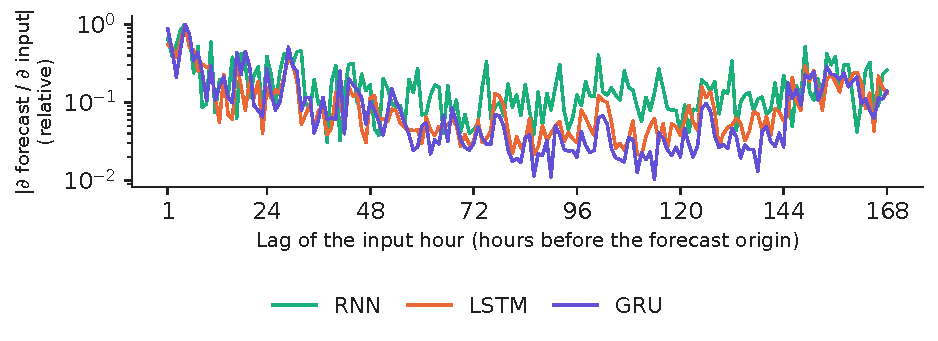
\includegraphics[width=\textwidth,height=0.324\textheight,keepaspectratio]{charts/en/grad_lag.pdf}\end{center}\vspace{-3mm}
\chartsource{Source: energy-charts.info (Fraunhofer ISE), from exchange and ENTSO-E data. Data: 200 test days of 2024; models with seed 20261108; forecast for noon (hour 12, universal time).}
\vspace{0.5mm}
\begin{itemize}\setlength{\itemsep}{0pt}
  \item Reading 7 daily profiles instead of 168 hours shortens the gradient path to 7 steps
    \begin{itemize}\setlength{\itemsep}{0pt}
      \item At a lag of one week the sensitivity, relative to the last day's maximum, is RNN 0.261, LSTM 0.131, GRU 0.140.
    \end{itemize}
\end{itemize}
\par\vfill\noindent{\scriptsize\color{FooterGray}(own computation)}\hfill\qlink{NN\_L5\_grad\_lag}{Quantlets/L5/NN_L5_grad_lag}\par\vspace{0.5mm}
\end{frame}

\begin{frame}{LSTM gates react to market stress}
\small
\intuition{gate activations of the trained volatility LSTM on the test years 2020--2026 (5-day means).}
\begin{center}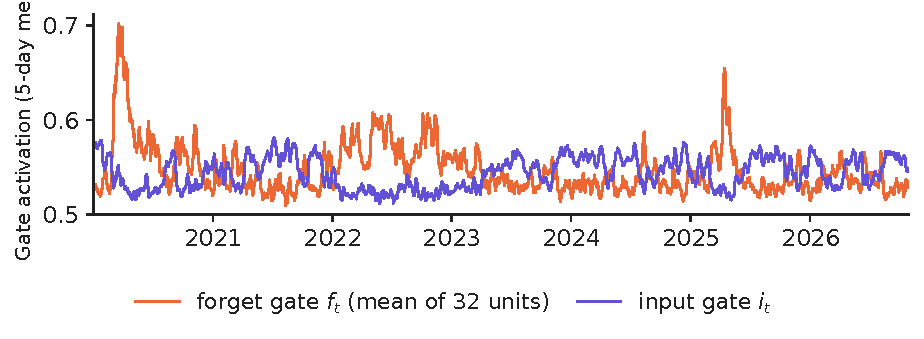
\includegraphics[width=\textwidth,height=0.420\textheight,keepaspectratio]{charts/en/lstm_gates.pdf}\end{center}\vspace{-3mm}
\chartsource{Source: Yahoo Finance, daily quotes. Data: test period 2020-2026, LSTM seed 20261108, last step of each 22-day window.}
\vspace{0.5mm}
\begin{itemize}\setlength{\itemsep}{0pt}
  \item Correlation with today's log variance: forget gate 0.743, input gate \ensuremath{-}0.616.
\end{itemize}
\par\vfill\manager{gates are a diagnostic, not an explanation: use them to see when the model changes regime, then check with the data.}\par\vspace{0.5mm}
\par\vfill\noindent{\scriptsize\color{FooterGray}(own computation)}\hfill\qlink{NN\_L5\_lstm\_gates}{Quantlets/L5/NN_L5_lstm_gates}\par\vspace{0.5mm}
\end{frame}

\begin{frame}{Sequence patterns and one trap}
\footnotesize
\begin{columns}[T,onlytextwidth]
\begin{column}{0.49\textwidth}
\begin{itemize}\setlength{\itemsep}{4pt}
  \item \textbf{Many-to-one}
    \begin{itemize}\setlength{\itemsep}{0pt}
      \item A window in, one value out: tomorrow's volatility
    \end{itemize}
  \item \textbf{Many-to-many (vector output)}
    \begin{itemize}\setlength{\itemsep}{0pt}
      \item A week of daily profiles in, 24 hours of tomorrow out: our load model
    \end{itemize}
  \item \textbf{Encoder--decoder}
    \begin{itemize}\setlength{\itemsep}{0pt}
      \item One network reads, another writes a sequence step by step
    \end{itemize}
\end{itemize}
\end{column}
\begin{column}{0.48\textwidth}
\begin{itemize}\setlength{\itemsep}{4pt}
  \item \textbf{Stacked}
    \begin{itemize}\setlength{\itemsep}{0pt}
      \item The states of layer 1 are the inputs of layer 2
    \end{itemize}
  \item \textbf{Bidirectional (BiLSTM)}
    \begin{itemize}\setlength{\itemsep}{0pt}
      \item Reads the window forward and backward
      \item Fine for classifying a finished text or sequence
      \item A leak in forecasting if the backward pass sees the future
    \end{itemize}
\end{itemize}
\end{column}
\end{columns}
\par\vfill\manager{in forecasting every input must be known at the forecast origin: check this before any architecture choice.}\par\vspace{0.5mm}
\par\vfill\noindent{\scriptsize\color{FooterGray}(Bishop \& Bishop, 2024, ch.~12)}\par\vspace{0.5mm}
\end{frame}


\section{A protocol for financial time series}

\begin{frame}{Windows, scaling and splits without leakage}
\footnotesize
\intuition{every number the model sees must be computable at the forecast origin $t$.}
\begin{columns}[T,onlytextwidth]
\begin{column}{0.53\textwidth}
\[ \mathcal D=\{(\mathbf x_{t-W+1:t},\,y_{t+1})\},\qquad \tilde x=\frac{x-\bar x_{\mathrm{train}}}{s_{\mathrm{train}}} \]{\footnotesize\begin{itemize}\setlength{\itemsep}{0pt}
  \item \textbf{\txtwhere}
    \begin{itemize}\setlength{\itemsep}{0pt}
      \item $W$ window
      \item $\bar x_{\mathrm{train}},s_{\mathrm{train}}$ mean and standard deviation of the training years only
    \end{itemize}
\end{itemize}\par}
\end{column}
\begin{column}{0.44\textwidth}
\begin{itemize}\setlength{\itemsep}{2pt}
  \item S\&P 500: 3\,020 training, 754 validation and 1\,717 test days, in this order.
  \item Early stopping: stop when the validation loss has not improved for 6 epochs
    \begin{itemize}\setlength{\itemsep}{0pt}
      \item Keep the best weights.
    \end{itemize}
  \item Seeds: 5 per network (volatility, returns), 3 for load
    \begin{itemize}\setlength{\itemsep}{0pt}
      \item We report the spread and the mean forecast.
    \end{itemize}
\end{itemize}
\end{column}
\end{columns}
\par\vfill\manager{a random shuffle of days before splitting puts 2020 in the training set and makes any model look good on 2020.}\par\vspace{0.5mm}
\par\vfill\noindent{\scriptsize\color{FooterGray}(own computation)}\hfill\tryit{\S2}\par\vspace{0.5mm}
\end{frame}

\begin{frame}{Benchmarks first: naive, HAR and GARCH}
\footnotesize
\intuition{a network must beat models that econometrics has refined for decades.}
\begin{columns}[T,onlytextwidth]
\begin{column}{0.53\textwidth}
\[\begin{aligned} \text{HAR: } y_{t+1}&=\beta_0+\beta_d y_t+\beta_w\bar y_{t-4:t}+\beta_m\bar y_{t-21:t}\\ \text{GARCH(1,1): } \sigma^2_{t+1}&=\omega+\alpha\,\varepsilon_t^2+\beta\,\sigma^2_t,\quad \varepsilon_t=r_t-\mu \end{aligned}\]{\footnotesize\begin{itemize}\setlength{\itemsep}{0pt}
  \item \textbf{\txtwhere}
    \begin{itemize}\setlength{\itemsep}{0pt}
      \item $y_t=\ln\hat\sigma^2_{\mathrm{GK},t}$
      \item $\bar y$ means over a week and a month
      \item GARCH with Student-$t$ errors, mapped to $y$ by a linear regression on the training years
      \item Naive: $\hat y_{t+1}=y_t$
    \end{itemize}
\end{itemize}\par}
\end{column}
\begin{column}{0.44\textwidth}
\begin{itemize}\setlength{\itemsep}{2pt}
  \item HAR estimates: $\hat\beta_d=0.192$, $\hat\beta_w=0.439$, $\hat\beta_m=0.293$.
  \item GARCH: $\hat\alpha=0.117$, $\hat\beta=0.873$, persistence 0.990, $\hat\nu=5.78$.
\end{itemize}
\end{column}
\end{columns}
\par\vfill\manager{HAR is a linear model with three averages
    \begin{itemize}\setlength{\itemsep}{0pt}
      \item If an LSTM cannot beat it, the LSTM is not worth maintaining.
    \end{itemize}}\par\vspace{0.5mm}
\par\vfill\noindent{\scriptsize\color{FooterGray}(Corsi, 2009; Bollerslev, 1986)}\par\vspace{0.5mm}
\end{frame}

\begin{frame}{Is one forecast really better? The Diebold--Mariano test}
\footnotesize
\intuition{compare the losses of two forecasts day by day and test whether their mean difference is zero.}
\begin{columns}[T,onlytextwidth]
\begin{column}{0.53\textwidth}
\[ d_t=L(e_{1,t})-L(e_{2,t}),\qquad \mathrm{DM}=\frac{\bar d}{\sqrt{\hat\sigma^2_{\mathrm{NW}}/n}}\;\overset{H_0}{\sim}\;\mathcal N(0,1) \]{\footnotesize\begin{itemize}\setlength{\itemsep}{0pt}
  \item \textbf{\txtwhere}
    \begin{itemize}\setlength{\itemsep}{0pt}
      \item $L$ squared error (volatility) or absolute error (load)
      \item $\hat\sigma^2_{\mathrm{NW}}$ Newey--West long-run variance of $d_t$
      \item $\mathrm{DM}<0$: model 1 better
    \end{itemize}
\end{itemize}\par}
\end{column}
\begin{column}{0.44\textwidth}
\begin{itemize}\setlength{\itemsep}{2pt}
  \item The Diebold--Mariano (DM) test accounts for autocorrelated loss differences, which forecast errors always have.
  \item Seeds measure the training noise
    \begin{itemize}\setlength{\itemsep}{0pt}
      \item DM measures the sampling noise of the test period.
    \end{itemize}
\end{itemize}
\end{column}
\end{columns}
\par\vfill\manager{report a model as better only with a DM $p$-value, and say over which period.}\par\vspace{0.5mm}
\par\vfill\noindent{\scriptsize\color{FooterGray}(Diebold \& Mariano, 1995)}\par\vspace{0.5mm}
\end{frame}


\section{Case study A: S\&P 500 volatility}

\begin{frame}{In the 2020 crash the LSTM adapted faster than HAR}
\small
\intuition{one-day-ahead forecasts of annualised volatility in the first test year.}
\vspace{-1mm}\[ \hat\sigma_{t+1}^{\mathrm{ann}}=100\sqrt{252\,\exp(\hat y_{t+1})} \]\vspace{-2mm}
\begin{center}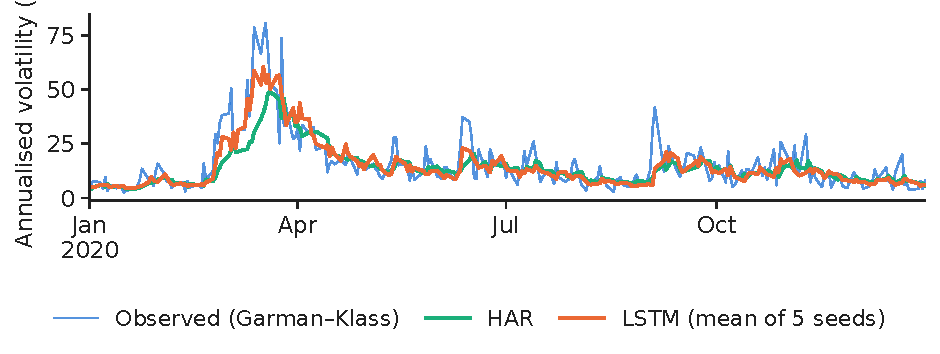
\includegraphics[width=\textwidth,height=0.420\textheight,keepaspectratio]{charts/en/vol_forecast.pdf}\end{center}\vspace{-3mm}
\chartsource{Source: Yahoo Finance, daily quotes. Data: test year 2020 (one-day-ahead forecasts), trading days.}
\vspace{0.5mm}
\begin{itemize}\setlength{\itemsep}{0pt}
  \item Crash window (20 Feb -- 30 Apr 2020), mean squared error (MSE) of $\hat y$: naive 0.705, GARCH 1.032, HAR 1.014, LSTM 0.521.
\end{itemize}
\par\vfill\noindent{\scriptsize\color{FooterGray}(own computation)}\hfill\qlink{NN\_L5\_vol\_forecast}{Quantlets/L5/NN_L5_vol_forecast}\par\vspace{0.5mm}
\end{frame}

\begin{frame}{Recurrent networks beat HAR and GARCH on volatility}
\small
\intuition{test MSE of the log variance over 2020--2026; dots are single seeds.}
\begin{center}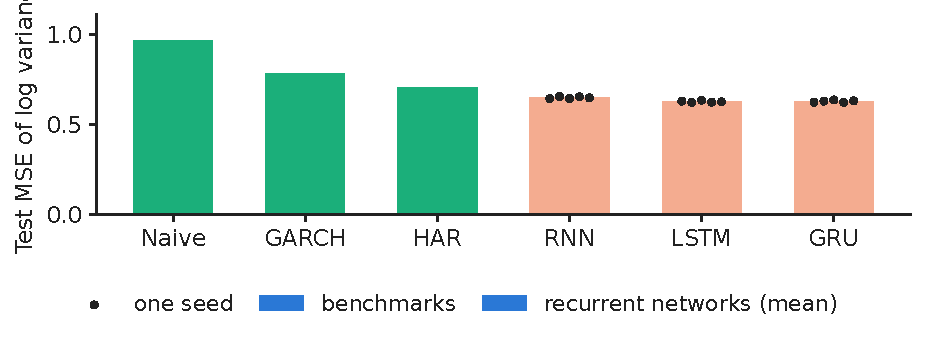
\includegraphics[width=\textwidth,height=0.420\textheight,keepaspectratio]{charts/en/vol_mse.pdf}\end{center}\vspace{-3mm}
\chartsource{Source: Yahoo Finance, daily quotes. Data: test 2 Jan 2020 to 31 Oct 2026; 5 seeds per network.}
\vspace{0.5mm}
\begin{itemize}\setlength{\itemsep}{0pt}
  \item MSE: naive 0.966, GARCH 0.786, HAR 0.706
    \begin{itemize}\setlength{\itemsep}{0pt}
      \item RNN 0.649, LSTM 0.628, GRU 0.629 (seed means).
    \end{itemize}
\end{itemize}
\par\vfill\noindent{\scriptsize\color{FooterGray}(own computation)}\hfill\qlink{NN\_L5\_vol\_mse}{Quantlets/L5/NN_L5_vol_mse}\par\vspace{0.5mm}
\end{frame}

\begin{frame}{Volatility results with tests}
\footnotesize
\begin{columns}[T,onlytextwidth]
\begin{column}{0.5\textwidth}
{\footnotesize\renewcommand{\arraystretch}{1.05}\setlength{\tabcolsep}{4pt}
\begin{tabular}{@{}lrrr@{}}\toprule
Model & MSE & $R^2$ & Seeds \\ \midrule
Naive & 0.966 & 0.259 & -- \\
GARCH(1,1)-$t$ & 0.786 & 0.397 & -- \\
HAR & 0.706 & 0.458 & -- \\
RNN (mean forecast) & 0.643 & 0.507 & 5 \\
LSTM (mean forecast) & 0.625 & 0.521 & 5 \\
GRU (mean forecast) & 0.624 & 0.521 & 5 \\
\bottomrule\end{tabular}}
\par\vspace{0.5mm}{\scriptsize \begin{itemize}\setlength{\itemsep}{0pt}
  \item $R^2=1-\mathrm{MSE}/\widehat{\Var}(y)$ on the 1\,717 test days.
\end{itemize}}
\end{column}
\begin{column}{0.47\textwidth}
\begin{itemize}\setlength{\itemsep}{4pt}
  \item LSTM vs HAR: MSE change \ensuremath{-}11.6\,\%
    \begin{itemize}\setlength{\itemsep}{0pt}
      \item DM $=\ensuremath{-}5.52$, $p<0.001$.
    \end{itemize}
  \item LSTM vs GARCH: DM $=\ensuremath{-}6.80$, $p<0.001$.
  \item LSTM vs naive: MSE change \ensuremath{-}35.3\,\%.
  \item Best network by mean forecast: GRU
    \begin{itemize}\setlength{\itemsep}{0pt}
      \item Seed spread of the LSTM: 0.623 to 0.635.
    \end{itemize}
\end{itemize}
\end{column}
\end{columns}
\par\vfill\manager{the gain is significant on this test period
    \begin{itemize}\setlength{\itemsep}{0pt}
      \item Before replacing HAR in a VaR model, check it on another market and sub-period and keep HAR as the fallback.
    \end{itemize}}\par\vspace{0.5mm}
\par\vfill\noindent{\scriptsize\color{FooterGray}(own computation)}\par\vspace{0.5mm}
\end{frame}


\section{Case study B: can a network forecast returns?}

\begin{frame}{Out of sample, return forecasts explain almost nothing}
\small
\intuition{next-day returns of the S\&P 500 and of Banca Transilvania (TLV) from the last 22 returns.}
\vspace{-1mm}\[ R^2_{\mathrm{OOS}}=1-\frac{\sum_{t\in\mathrm{test}}(r_{t+1}-\hat r_{t+1})^2}{\sum_{t\in\mathrm{test}}r_{t+1}^2} \]\vspace{-2mm}
\begin{center}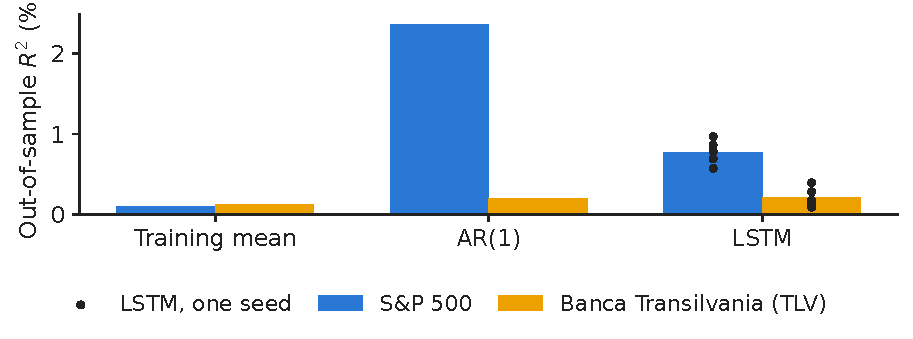
\includegraphics[width=\textwidth,height=0.384\textheight,keepaspectratio]{charts/en/returns_r2.pdf}\end{center}\vspace{-3mm}
\chartsource{Source: Yahoo Finance; EODHD. Data: test 2020 to Oct 2026; S\&P 500 (Yahoo Finance) and TLV (EODHD, Bucharest Stock Exchange).}
\vspace{0.5mm}
\begin{itemize}\setlength{\itemsep}{0pt}
  \item S\&P 500: AR(1) 2.366\,\%, LSTM 0.776\,\% (seeds 0.572 to 0.969)
    \begin{itemize}\setlength{\itemsep}{0pt}
      \item TLV: AR(1) 0.201\,\%, LSTM 0.213\,\%.
    \end{itemize}
\end{itemize}
\par\vfill\noindent{\scriptsize\color{FooterGray}(own computation)}\hfill\qlink{NN\_L5\_returns\_r2}{Quantlets/L5/NN_L5_returns_r2}\par\vspace{0.5mm}
\end{frame}

\begin{frame}{Why return forecasts stay weak, and what that teaches}
\footnotesize
\intuition{in a liquid market the predictable part of returns is tiny compared with their noise.}
\begin{columns}[T,onlytextwidth]
\begin{column}{0.53\textwidth}
\[ r_{t+1}=\mu_t+\varepsilon_{t+1},\qquad \frac{\Var(\mu_t)}{\Var(r_{t+1})}\approx0 \]{\footnotesize\begin{itemize}\setlength{\itemsep}{0pt}
  \item \textbf{\txtwhere}
    \begin{itemize}\setlength{\itemsep}{0pt}
      \item $\mu_t$ the conditional mean a model can learn
      \item $\varepsilon_{t+1}$ news that arrives after $t$
    \end{itemize}
\end{itemize}\par}
\end{column}
\begin{column}{0.44\textwidth}
\begin{itemize}\setlength{\itemsep}{2pt}
  \item LSTM sign accuracy on the S\&P 500 test: 52.1\,\%, against 54.0\,\% up days (always ``up'').
  \item AR(1) slope estimated on the training years: \ensuremath{-}0.102 (S\&P 500), 0.015 (TLV).
  \item Flexible models fit noise in training
    \begin{itemize}\setlength{\itemsep}{0pt}
      \item Early stopping limits the damage, it cannot create a signal.
    \end{itemize}
\end{itemize}
\end{column}
\end{columns}
\par\vfill\manager{a vendor's back-test of an ``artificial intelligence (AI) return predictor'' must pass this test on data it has never seen, after costs.}\par\vspace{0.5mm}
\par\vfill\noindent{\scriptsize\color{FooterGray}(own computation)}\par\vspace{0.5mm}
\end{frame}


\section{Case study C: Romanian electricity load}

\begin{frame}{Load has daily, weekly and yearly cycles}
\small
\intuition{a sequence with long, regular memory: a natural case for recurrent networks.}
\begin{center}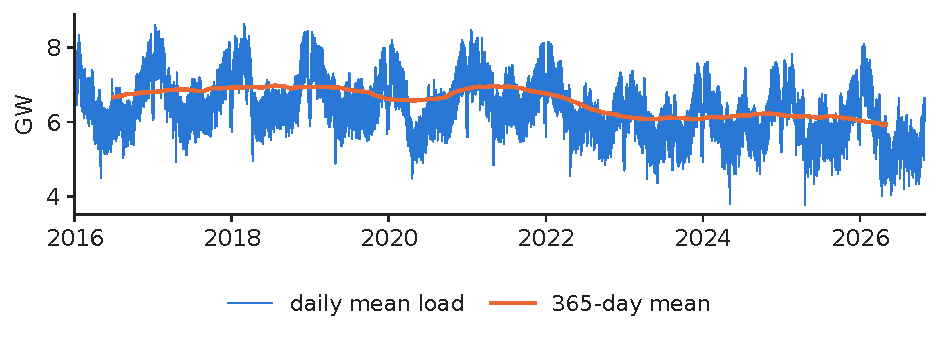
\includegraphics[width=\textwidth,height=0.420\textheight,keepaspectratio]{charts/en/load_series.pdf}\end{center}\vspace{-3mm}
\chartsource{Source: energy-charts.info (Fraunhofer ISE), from exchange and ENTSO-E data. Data: 1 Jan 2016 to 31 Oct 2026, hourly, mean MW per day.}
\vspace{0.5mm}
\begin{itemize}\setlength{\itemsep}{0pt}
  \item Hourly load from 1 Jan 2016 to 31 Oct 2026, mean 6\,510 megawatt (MW)
    \begin{itemize}\setlength{\itemsep}{0pt}
      \item 129 missing hours stay missing (those days are skipped).
    \end{itemize}
\end{itemize}
\par\vfill\noindent{\scriptsize\color{FooterGray}(own computation)}\hfill\qlink{NN\_L5\_load\_series}{Quantlets/L5/NN_L5_load_series}\par\vspace{0.5mm}
\end{frame}

\begin{frame}{The day-ahead task and its benchmarks}
\scriptsize
\intuition{at the end of day $d$ forecast the 24 hourly loads of day $d+1$ from the last week.}
\begin{columns}[T,onlytextwidth]
\begin{column}{0.64\textwidth}
\[ \hat{\mathbf y}_{d+1}=\mathbf y_{d-6}+\mW_{o}[\vh_{7};\mathbf s_{d+1}]+\vb_o\in\R^{24} \]\vspace{-2mm}\[ \text{ARX: } \hat{\mathbf y}_{d+1}=\mathbf y_{d-6}+\mathbf B\,\mathbf x_{d,1:168}+\mathbf\Gamma\mathbf s_{d+1} \]{\footnotesize\begin{itemize}\setlength{\itemsep}{0pt}
  \item \textbf{\txtwhere}
    \begin{itemize}\setlength{\itemsep}{0pt}
      \item $\mathbf y_{d-6}$ seasonal naive forecast (the models learn its correction)
      \item $\vh_{7}$ last state after the 7 past days, one step per day (24 hourly loads + weekday)
      \item $\mathbf s_{d+1}$ weekday and season of day $d+1$
      \item ARX by ridge regression (penalty 1, chosen on the validation year)
    \end{itemize}
\end{itemize}\par}
\end{column}
\begin{column}{0.33\textwidth}
\begin{itemize}\setlength{\itemsep}{2pt}
  \item 2\,186 training, 365 validation, 1035 test days
    \begin{itemize}\setlength{\itemsep}{0pt}
      \item 3 seeds per network.
    \end{itemize}
\end{itemize}
\end{column}
\end{columns}
\par\vfill\manager{a supplier submits the 24 hourly volumes before noon
    \begin{itemize}\setlength{\itemsep}{0pt}
      \item Every MW of error is bought or sold at the imbalance price.
    \end{itemize}}\par\vspace{0.5mm}
\par\vfill\noindent{\scriptsize\color{FooterGray}(own computation)}\hfill\tryit{\S5}\par\vspace{0.5mm}
\end{frame}

\begin{frame}{Two winter test weeks: forecasts against the observed load}
\small
\intuition{hourly load in two winter test weeks, observed against two forecasts.}
\begin{center}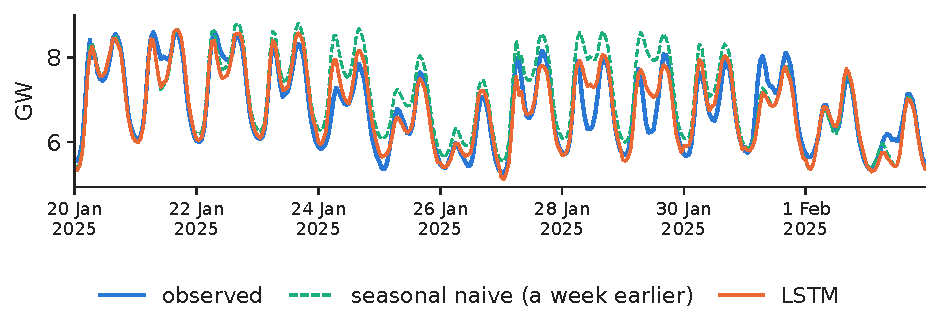
\includegraphics[width=\textwidth,height=0.450\textheight,keepaspectratio]{charts/en/load_fortnight.pdf}\end{center}\vspace{-3mm}
\chartsource{Source: energy-charts.info (Fraunhofer ISE), from exchange and ENTSO-E data. Data: 14 test days from 20 Jan 2025 to 2 Feb 2025.}
\vspace{0.5mm}
\begin{itemize}\setlength{\itemsep}{0pt}
  \item The seasonal naive copies last week, including its level and its holidays
    \begin{itemize}\setlength{\itemsep}{0pt}
      \item The networks learn only a correction of it.
    \end{itemize}
\end{itemize}
\par\vfill\noindent{\scriptsize\color{FooterGray}(own computation)}\hfill\qlink{NN\_L5\_load\_fortnight}{Quantlets/L5/NN_L5_load_fortnight}\par\vspace{0.5mm}
\end{frame}

\begin{frame}{On load, the linear ARX beats the recurrent networks}
\small
\intuition{left: mean absolute percentage error (MAPE) over all test hours; right: mean absolute error (MAE) by hour of day.}
\vspace{-1mm}\[ \mathrm{MAPE}=\frac{100}{24n}\sum_{d}\sum_{h=1}^{24}\frac{|y_{d,h}-\hat y_{d,h}|}{y_{d,h}} \]\vspace{-2mm}
\begin{center}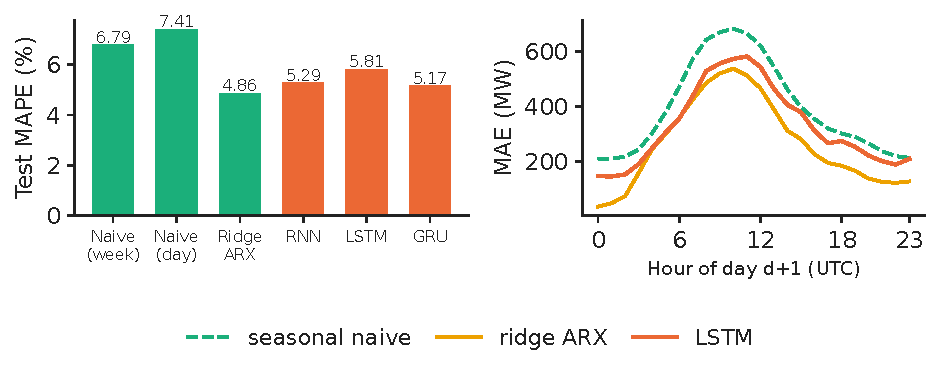
\includegraphics[width=\textwidth,height=0.420\textheight,keepaspectratio]{charts/en/load_errors.pdf}\end{center}\vspace{-3mm}
\chartsource{Source: energy-charts.info (Fraunhofer ISE), from exchange and ENTSO-E data. Data: 1 Jan 2024 to 31 Oct 2026 (test days).}
\vspace{0.5mm}
\begin{itemize}\setlength{\itemsep}{0pt}
  \item MAPE (\%): seasonal naive 6.79, naive 7.41, ridge ARX 4.86, RNN 5.29, LSTM 5.81, GRU 5.17.
\end{itemize}
\par\vfill\noindent{\scriptsize\color{FooterGray}(own computation)}\hfill\qlink{NN\_L5\_load\_errors}{Quantlets/L5/NN_L5_load_errors}\par\vspace{0.5mm}
\end{frame}

\begin{frame}{Longer windows help the LSTM, up to a week}
\small
\intuition{LSTM test error as a function of the input window, same protocol otherwise.}
\begin{center}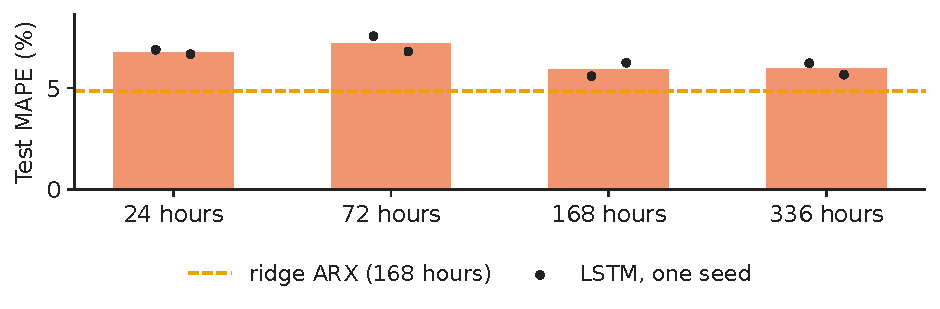
\includegraphics[width=\textwidth,height=0.420\textheight,keepaspectratio]{charts/en/load_window.pdf}\end{center}\vspace{-3mm}
\chartsource{Source: energy-charts.info (Fraunhofer ISE), from exchange and ENTSO-E data. Data: test days 2024-2026; LSTM with 2 seeds per window.}
\vspace{0.5mm}
\begin{itemize}\setlength{\itemsep}{0pt}
  \item MAPE (\%): 24 hours 6.77, 72 hours 7.17, 168 hours 5.91, 336 hours 5.93.
\end{itemize}
\par\vfill\noindent{\scriptsize\color{FooterGray}(own computation)}\hfill\qlink{NN\_L5\_load\_window}{Quantlets/L5/NN_L5_load_window}\par\vspace{0.5mm}
\end{frame}

\begin{frame}{What a better load forecast is worth}
\footnotesize
\begin{itemize}\setlength{\itemsep}{4pt}
  \item \textbf{Significance}
    \begin{itemize}\setlength{\itemsep}{0pt}
      \item Best network by mean forecast: GRU, MAPE \ensuremath{+}6.4\,\% relative to ridge ARX: with 2\,186 training days the linear model wins
      \item DM on daily MAE, LSTM vs ridge ARX: 9.80, $p<0.001$
    \end{itemize}
  \item \textbf{In megawatts}
    \begin{itemize}\setlength{\itemsep}{0pt}
      \item Mean absolute error per hour: seasonal naive 396 MW, ridge ARX 269 MW, LSTM 331 MW
      \item LSTM instead of the seasonal naive: about 1\,560 megawatt-hours (MWh) less absolute error per day, at national scale
    \end{itemize}
  \item \textbf{Cost}
    \begin{itemize}\setlength{\itemsep}{0pt}
      \item Training of all load models and the window study: 67 seconds on a laptop CPU
    \end{itemize}
\end{itemize}
\par\vfill\manager{multiply the MWh saved by the imbalance price spread and compare with the cost of the model: here the ridge ARX saves the most for the least
    \begin{itemize}\setlength{\itemsep}{0pt}
      \item Weather inputs would add more (Lecture 13).
    \end{itemize}}\par\vspace{0.5mm}
\par\vfill\noindent{\scriptsize\color{FooterGray}(own computation)}\par\vspace{0.5mm}
\end{frame}

\section*{Wrap-up}

\begin{frame}{Quiz 1: parameters}
\small
\begin{itemize}
  \item How many parameters has an LSTM layer with $d=3$ inputs and $n_h=32$ units?
\end{itemize}
\vspace{2mm}
\begin{exampleblock}{Answer}
\begin{itemize}
  \item $4n_h(n_h+d+1)=4\cdot32\cdot36=4608$ (PyTorch keeps two bias vectors, so it reports $4608+128=4736$).
\end{itemize}
\end{exampleblock}
\end{frame}

\begin{frame}{Quiz 2: gradients}
\small
\begin{itemize}
  \item Why does a vanilla RNN struggle with the weekly pattern of hourly load?
\end{itemize}
\vspace{2mm}
\begin{exampleblock}{Answer}
\begin{itemize}
  \item Over 168 hourly steps the gradient is a product of 168 Jacobians and vanishes
    \begin{itemize}\setlength{\itemsep}{0pt}
      \item Reading 7 daily profiles shortens the path to 7 steps, which is how our load models are built.
    \end{itemize}
\end{itemize}
\end{exampleblock}
\end{frame}

\begin{frame}{Quiz 3: a vendor's claim}
\small
\begin{itemize}
  \item A vendor shows an LSTM with 60\,\% sign accuracy on S\&P 500 returns, trained on shuffled days
    \begin{itemize}\setlength{\itemsep}{0pt}
      \item What do you ask?
    \end{itemize}
\end{itemize}
\vspace{2mm}
\begin{exampleblock}{Answer}
\begin{itemize}
  \item A time-ordered test on unseen years, against ``always up'' (54.0\,\%) and after costs
    \begin{itemize}\setlength{\itemsep}{0pt}
      \item Our honest LSTM reaches 52.1\,\%.
    \end{itemize}
\end{itemize}
\end{exampleblock}
\end{frame}

\begin{frame}{Quiz 4: HAR or LSTM}
\small
\begin{itemize}
  \item The LSTM changes the volatility MSE by \ensuremath{-}11.6\,\% against HAR, with DM $=\ensuremath{-}5.52$
    \begin{itemize}\setlength{\itemsep}{0pt}
      \item Does it replace HAR in the VaR system?
    \end{itemize}
\end{itemize}
\vspace{2mm}
\begin{exampleblock}{Answer}
\begin{itemize}
  \item The gain is significant here, so the LSTM is a serious candidate
    \begin{itemize}\setlength{\itemsep}{0pt}
      \item Switch only after it holds on another market and sub-period, with monitoring and HAR as the fallback.
    \end{itemize}
\end{itemize}
\end{exampleblock}
\end{frame}

\begin{frame}{Quiz 5: bidirectional}
\small
\begin{itemize}
  \item Can you use a bidirectional LSTM to forecast tomorrow's load from a window that ends today?
\end{itemize}
\vspace{2mm}
\begin{exampleblock}{Answer}
\begin{itemize}
  \item Yes, if the window ends at the forecast origin: the backward pass then sees only the past
    \begin{itemize}\setlength{\itemsep}{0pt}
      \item It leaks only if the window contains hours after the origin.
    \end{itemize}
\end{itemize}
\end{exampleblock}
\end{frame}

\begin{frame}{Wrap-up}
\small
\vspace{-2mm}\begin{multicols}{2}\scriptsize\tableofcontents\end{multicols}
\begin{itemize}\setlength{\itemsep}{1pt}
  \item An RNN shares weights in time
    \begin{itemize}\setlength{\itemsep}{0pt}
      \item BPTT multiplies Jacobians, so gradients vanish or explode
      \item LSTM and GRU add an additive memory path.
    \end{itemize}
  \item On real data: the networks beat HAR on volatility, return forecasts explain almost nothing, and a linear ARX wins on hourly load.
    \begin{itemize}\setlength{\itemsep}{0pt}
      \item Next: text (Lecture 6).
    \end{itemize}
\end{itemize}
\end{frame}

\begin{frame}{Research from our group: sequences and risk}
\footnotesize
\begin{itemize}\setlength{\itemsep}{3pt}
  \item \textbf{Can foundation models manage risk?} (Jheng, Tak, Găman, Mazurencu-Marinescu-Pele \& Pele, 2026, Economic Computation and Economic Cybernetics Studies and Research)
    \begin{itemize}\setlength{\itemsep}{0pt}
      \item Pre-trained time-series models used without fine-tuning to forecast VaR and expected shortfall (ES) for Central and Eastern European (CEE) markets
      \item A conformal calibration step makes the tail forecasts reliable; the transformer successors of the LSTM come in Lectures 7 and 13
    \end{itemize}
  \item \textbf{Early warning of ``zombie'' crypto-assets} (Będowska-Sójka, Wójcik \& Pele, 2026, North American Journal of Economics and Finance)
    \begin{itemize}\setlength{\itemsep}{0pt}
      \item A machine-learning early-warning system for crypto-assets that lose their market activity
    \end{itemize}
  \item \textbf{BitMood} (Conda, Găman, Bâg, Mazurencu-Marinescu-Pele, Pele \& Härdle, 2026, Digital Finance)
    \begin{itemize}\setlength{\itemsep}{0pt}
      \item Facebook sentiment and Bitcoin volume: linear regression and a bidirectional LSTM reach comparable test performance, so model complexity does not guarantee better forecasts
    \end{itemize}
\end{itemize}
\par\vspace{0.5mm}{\scriptsize \begin{itemize}\setlength{\itemsep}{0pt}
  \item Findings as stated in the papers; numbers on the other slides come from our own computations.
\end{itemize}}
\par\vfill\noindent{\scriptsize\color{FooterGray}(Bucharest University of Economic Studies; Romanian Academy, Institute for Economic Forecasting)}\par\vspace{0.5mm}
\end{frame}

\begin{frame}{Want to learn more?}
\small
\begin{columns}[T,onlytextwidth]
\begin{column}{0.52\textwidth}
\begin{itemize}\setlength{\itemsep}{4pt}
  \item \textbf{Bishop \& Bishop (2024)}, ch.~12: sequence models, from RNNs to transformers.
  \item \textbf{Pascanu, Mikolov \& Bengio (2013)}: the clearest analysis of vanishing and exploding gradients.
  \item \textbf{Corsi (2009)}: the HAR model, the benchmark every volatility network must face.
\end{itemize}
\end{column}
\begin{column}{0.45\textwidth}
\begin{itemize}\setlength{\itemsep}{4pt}
  \item \textbf{This course}: code, data, notebooks --- \href{https://github.com/danpele/NEURAL_BIZ}{github.com/danpele/NEURAL\_BIZ}.
  \item \textbf{Experiment yourself}: the notebook reproduces the charts of this lecture --- \href{\nnrepo/\nnnb}{notebooks/}.
  \item \textbf{Seminar 5}: a GRU for the volatility of another index, against HAR, with a DM test.
\end{itemize}
\end{column}
\end{columns}
\end{frame}

\begin{frame}{References (1/2)}
\scriptsize
\begin{itemize}\setlength{\itemsep}{0pt}\scriptsize
\item Bengio, Y., Simard, P.\ \& Frasconi, P.\ (1994). Learning long-term dependencies with gradient descent is difficult. \textit{IEEE Transactions on Neural Networks}, 5(2), 157--166. \href{https://doi.org/10.1109/72.279181}{doi:10.1109/72.279181}
\item Bishop, C.\,M.\ \& Bishop, H.\ (2024). \textit{Deep Learning: Foundations and Concepts}, ch.~12. Springer. \href{https://doi.org/10.1007/978-3-031-45468-4}{doi:10.1007/978-3-031-45468-4}
\item Bollerslev, T.\ (1986). Generalized autoregressive conditional heteroskedasticity. \textit{Journal of Econometrics}, 31(3), 307--327. \href{https://doi.org/10.1016/0304-4076(86)90063-1}{doi:10.1016/0304-4076(86)90063-1}
\item Będowska-Sójka, B., Wójcik, P.\ \& Pele, D.\,T.\ (2026). Early warning systems for cryptocurrency markets: Predicting `zombie' assets using machine learning. \textit{North American Journal of Economics and Finance}, 81, 102543. \href{https://doi.org/10.1016/j.najef.2025.102543}{doi:10.1016/j.najef.2025.102543}
\item Cho, K., van Merriënboer, B., Gulcehre, C., Bahdanau, D., Bougares, F., Schwenk, H.\ \& Bengio, Y.\ (2014). Learning phrase representations using RNN encoder--decoder for statistical machine translation. \textit{EMNLP}, 1724--1734. \href{https://doi.org/10.3115/v1/D14-1179}{doi:10.3115/v1/D14-1179}
\item Conda, A.\,I., Găman, Ș., Bâg, R.\,C., Mazurencu-Marinescu-Pele, M., Pele, D.\,T.\ \& Härdle, W.\,K.\ (2026). BitMood: AI analysis of Bitcoin trends via Facebook emotions. \textit{Digital Finance}, 8(3), 42. \href{https://doi.org/10.1007/s42521-026-00205-3}{doi:10.1007/s42521-026-00205-3}
\item Corsi, F.\ (2009). A simple approximate long-memory model of realized volatility. \textit{Journal of Financial Econometrics}, 7(2), 174--196. \href{https://doi.org/10.1093/jjfinec/nbp001}{doi:10.1093/jjfinec/nbp001}
\item Diebold, F.\,X.\ \& Mariano, R.\,S.\ (1995). Comparing predictive accuracy. \textit{Journal of Business \& Economic Statistics}, 13(3), 253--263. \href{https://doi.org/10.1080/07350015.1995.10524599}{doi:10.1080/07350015.1995.10524599}
\end{itemize}
\end{frame}

\begin{frame}{References (2/2)}
\scriptsize
\begin{itemize}\setlength{\itemsep}{0pt}\scriptsize
\item Garman, M.\,B.\ \& Klass, M.\,J.\ (1980). On the estimation of security price volatilities from historical data. \textit{Journal of Business}, 53(1), 67--78. \href{https://doi.org/10.1086/296072}{doi:10.1086/296072}
\item Hochreiter, S.\ \& Schmidhuber, J.\ (1997). Long short-term memory. \textit{Neural Computation}, 9(8), 1735--1780. \href{https://doi.org/10.1162/neco.1997.9.8.1735}{doi:10.1162/neco.1997.9.8.1735}
\item Jheng, S.-L., Tak, R., Găman, Ș., Mazurencu-Marinescu-Pele, M.\ \& Pele, D.\,T.\ (2026). Can foundation models manage risk? Zero-shot VaR and ES forecasting with conformal calibration in CEE markets. \textit{Economic Computation and Economic Cybernetics Studies and Research}, 60(2), 267--290. \href{https://doi.org/10.24818/18423264/60.2.26.14}{doi:10.24818/18423264/60.2.26.14}
\item Pascanu, R., Mikolov, T.\ \& Bengio, Y.\ (2013). On the difficulty of training recurrent neural networks. \textit{ICML}, PMLR 28(3), 1310--1318. \href{https://arxiv.org/abs/1211.5063}{arXiv:1211.5063}
\item Rumelhart, D.\,E., Hinton, G.\,E.\ \& Williams, R.\,J.\ (1986). Learning representations by back-propagating errors. \textit{Nature}, 323, 533--536. \href{https://doi.org/10.1038/323533a0}{doi:10.1038/323533a0}
\item Werbos, P.\,J.\ (1990). Backpropagation through time: What it does and how to do it. \textit{Proceedings of the IEEE}, 78(10), 1550--1560. \href{https://doi.org/10.1109/5.58337}{doi:10.1109/5.58337}
\end{itemize}
\end{frame}

\appendix

\begin{frame}{Appendix: BPTT for the vanilla RNN, step by step}
\footnotesize
\begin{itemize}\setlength{\itemsep}{3pt}
  \item Pre-activation $\mathbf a_t=\mW_{xh}\vx_t+\mW_{hh}\vh_{t-1}+\vb_h$, state $\vh_t=\tanh(\mathbf a_t)$, loss $\loss=\sum_t\ell_t(\hat y_t,y_t)$.
  \item Backward recursion: $\boldsymbol\delta_t\equiv\partial\loss/\partial\vh_t=\mW_{hy}^{\top}\partial\ell_t/\partial\hat y_t+\mW_{hh}^{\top}\big[(1-\vh_{t+1}^2)\odot\boldsymbol\delta_{t+1}\big]$, with $\boldsymbol\delta_{T+1}=\mathbf 0$.
  \item Weight gradients: $\partial\loss/\partial\mW_{hh}=\sum_t\big[(1-\vh_t^2)\odot\boldsymbol\delta_t\big]\vh_{t-1}^{\top}$, $\partial\loss/\partial\mW_{xh}=\sum_t\big[(1-\vh_t^2)\odot\boldsymbol\delta_t\big]\vx_t^{\top}$.
  \item Unrolling the recursion gives the product of Jacobians of the main text
    \begin{itemize}\setlength{\itemsep}{0pt}
      \item Many-to-one models have $\partial\ell_t/\partial\hat y_t=0$ for $t<T$.
    \end{itemize}
\end{itemize}
\end{frame}

\begin{frame}{Appendix: the models in PyTorch}
\footnotesize
{\scriptsize\ttfamily\setlength{\parindent}{0pt}class RecNet(nn.Module):\\
\hspace*{2.0em}def \_\_init\_\_(self, cell, n\_in, hidden=32, n\_out=1, n\_static=0):\\
\hspace*{4.0em}super().\_\_init\_\_()\\
\hspace*{4.0em}self.rnn = \{'rnn': nn.RNN, 'lstm': nn.LSTM, 'gru': nn.GRU\}[cell](n\_in, hidden, batch\_first=True)\\
\hspace*{4.0em}self.out = nn.Linear(hidden + n\_static, n\_out)\\
\hspace*{2.0em}def forward(self, x, s=None):\ \ \ \ \ \ \ \ \ \ \ \ \ \ \ \  \# x: batch x time x features\\
\hspace*{4.0em}h, \_ = self.rnn(x)\\
\hspace*{4.0em}z = h[:, -1] if s is None else torch.cat([h[:, -1], s], 1)\\
\hspace*{4.0em}return self.out(z)\\
\# training step: loss.backward(); nn.utils.clip\_grad\_norm\_(model.parameters(), 1.0); opt.step()\par}\begin{itemize}\setlength{\itemsep}{2pt}
  \item Full code: lectures/L5/analysis\_L5.py and the notebook of this lecture.
\end{itemize}
\end{frame}

\end{document}
